\documentclass[10pt]{article}
% paper/supp_style.tex - shared layout of the CUTLINE Supplementary Material (supplement.tex) and the online
% Reproducibility Report (reproducibility_report.tex). Figures follow paper/figs/src/cutline_style.py (sans, one accent
% colour for CUTLINE, greys for baselines); this file gives the text the same accent and a quiet sans heading style.
\usepackage[letterpaper,margin=0.85in,headheight=14pt,headsep=14pt,footskip=26pt]{geometry}
\usepackage[T1]{fontenc}
\usepackage{cite}
\usepackage{amsmath,amssymb}
\usepackage{amsthm}
\usepackage{newtxtext,newtxmath}
\setsansfont{texgyreheros-regular.otf}[BoldFont=texgyreheros-bold.otf,ItalicFont=texgyreheros-italic.otf,
  BoldItalicFont=texgyreheros-bolditalic.otf,Scale=MatchLowercase]
\usepackage{xeCJK}\setCJKmainfont{FandolSong-Regular.otf}[BoldFont=FandolSong-Bold.otf]
\usepackage{graphicx}
\usepackage{booktabs}
\usepackage{array}
\usepackage{tabularx}
\usepackage{multirow}
\usepackage{longtable}
\usepackage{pdflscape}
\usepackage{xcolor}
\usepackage{tikz}
\usetikzlibrary{arrows.meta,positioning,fit,backgrounds,calc}
\usepackage{xurl}
\usepackage{microtype}
\usepackage[shortlabels]{enumitem}
\usepackage{titlesec}
\usepackage[titles]{tocloft}
\usepackage{fancyhdr}
\usepackage{caption}
\usepackage{xr-hyper}
\usepackage[colorlinks=true,linkcolor=cutlink,citecolor=cutlink,urlcolor=cutlink,bookmarksnumbered=true,
  bookmarksopen=true,bookmarksopenlevel=1,pdfdisplaydoctitle=true]{hyperref}
\usepackage{bookmark}

% ---- colours (cutline_style.C) ----
\definecolor{cutaccent}{HTML}{1F5FAD}
\definecolor{cutaccentlight}{HTML}{C9DAF1}
\definecolor{cutlink}{HTML}{1B4F8F}
\definecolor{cutgrey}{HTML}{4D4D4D}
\definecolor{cutgreylight}{HTML}{ECECEC}
\definecolor{cutgen}{HTML}{E69F00}
\definecolor{cutgenlight}{HTML}{FBE3B0}
\definecolor{cutfail}{HTML}{D1495B}
\definecolor{cutfaillight}{HTML}{F6CDD2}
\definecolor{cutledger}{HTML}{7A5195}
\definecolor{cutledgerlight}{HTML}{E6DCEF}

% ---- headings: sans, accent rule under sections ----
\titleformat{\part}[block]{\sffamily\bfseries\Large\color{cutaccent}}{Part~\thepart}{0.6em}{}[\vspace{2pt}{\color{cutaccent}\titlerule[0.8pt]}]
\titlespacing*{\part}{0pt}{16pt}{10pt}
\titleformat{\section}{\sffamily\bfseries\large}{\thesection}{0.7em}{}
\titlespacing*{\section}{0pt}{14pt plus 3pt minus 2pt}{6pt plus 2pt}
\titleformat{\subsection}{\sffamily\bfseries\normalsize}{\thesubsection}{0.7em}{}
\titlespacing*{\subsection}{0pt}{10pt plus 2pt minus 2pt}{4pt plus 1pt}
\titleformat{\paragraph}[runin]{\sffamily\bfseries\small}{}{0pt}{}[.]
\titlespacing*{\paragraph}{0pt}{6pt plus 2pt}{0.6em}
\renewcommand{\thepart}{\Alph{part}}

% ---- running head ----
\newcommand{\runninghead}{}
\pagestyle{fancy}\fancyhf{}
\renewcommand{\headrulewidth}{0.4pt}\renewcommand{\headrule}{{\color{cutgreylight}\hrule height\headrulewidth}}
\fancyhead[L]{\sffamily\footnotesize\color{cutgrey}\textsc{Cutline}\enspace\textperiodcentered\enspace\runninghead}
\fancyhead[R]{\sffamily\footnotesize\color{cutgrey}\thepage}
\fancypagestyle{plain}{\fancyhf{}\renewcommand{\headrulewidth}{0pt}\fancyfoot[C]{\sffamily\footnotesize\color{cutgrey}\thepage}}

% ---- captions: tables above (IEEE), figures below; bold label, the first sentence of each caption is its title ----
\DeclareCaptionLabelFormat{ieeetab}{\textsc{Table}~#2}
\captionsetup{font=small,labelfont={bf},labelsep=period,justification=justified,singlelinecheck=true}
\captionsetup[figure]{name=Fig.,skip=6pt}
\captionsetup[table]{labelformat=ieeetab,position=top,skip=4pt}
\newcommand{\tabnote}[1]{\par\smallskip{\footnotesize\raggedright#1\par}}

% ---- tables ----
\renewcommand{\arraystretch}{1.12}
\setlength{\aboverulesep}{0.3ex}\setlength{\belowrulesep}{0.5ex}
\newcolumntype{L}[1]{>{\raggedright\arraybackslash}p{#1}}
\newcolumntype{Y}{>{\raggedright\arraybackslash}X}
\newcommand{\tabsize}{\fontsize{8}{9.6}\selectfont}
\newcommand{\tabsmall}{\fontsize{7.2}{8.6}\selectfont}

% ---- theorems and proofs in the style of the manuscript (IEEEtran: italic "Name n (note):", upright body) ----
\newtheoremstyle{ieee}{4pt plus 2pt}{4pt plus 2pt}{\upshape}{\parindent}{\itshape}{:}{0.5em}%
  {\thmname{#1}\thmnumber{ #2}\thmnote{ (#3)}}
\theoremstyle{ieee}
\makeatletter
\renewenvironment{proof}[1][\proofname]{\par\pushQED{\qed}\normalfont\topsep4pt plus 2pt\trivlist
  \item[\hskip\labelsep\hskip\parindent\itshape#1:]\ignorespaces}{\popQED\endtrivlist\@endpefalse}
\makeatother
\renewcommand{\qedsymbol}{$\square$}

% ---- typography ----
\widowpenalty=10000\clubpenalty=10000\displaywidowpenalty=10000
\setlist{itemsep=2pt,topsep=3pt,parsep=0pt,leftmargin=1.4em}
\setcounter{tocdepth}{2}
\setlength{\cftsecnumwidth}{2.6em}\setlength{\cftsubsecnumwidth}{3.3em}\setlength{\cftsubsecindent}{2.6em}
\renewcommand{\cftpartfont}{\sffamily\bfseries\color{cutaccent}}\renewcommand{\cftpartpagefont}{\sffamily\bfseries\color{cutaccent}}
\renewcommand{\cftsecfont}{\sffamily\bfseries}\renewcommand{\cftsecpagefont}{\sffamily\bfseries}
\renewcommand{\cfttoctitlefont}{\sffamily\bfseries\large}\setlength{\cftbeforesecskip}{2pt}\setlength{\cftbeforepartskip}{8pt}
\renewcommand{\cftpartpresnum}{Part~}\setlength{\cftpartnumwidth}{4.2em}
\renewcommand{\floatpagefraction}{0.8}\renewcommand{\topfraction}{0.9}\renewcommand{\textfraction}{0.08}
\setcounter{topnumber}{3}
\providecommand{\mainrefx}[1]{\ref*{M-#1}}

\newcommand{\sys}{\textsc{Cutline}}
% \cutid{...}: every in-text identifier (levels G0-G4, evidence tiers X0/X1/XP/T, assumptions AS1-AS10, threats T1-T7,
% residuals RF0-RF5, workflows WF1-WF3, oracles and algorithms). Upright sans (TeX Gyre Heros, the Helvetica clone that
% matches the Arial-metric figure text), never small caps, never hyphenated.
\providecommand{\cutid}[1]{\mbox{\sffamily\upshape #1}}
\newcommand{\G}[1]{\cutid{G#1}}
% Evidence tiers. They were called E0/E1/EP in the code and the registration files; the paper calls them X0/X1/XP so
% that they cannot be confused with the experiment identifiers E1-E21.
\newcommand{\Ezero}{\cutid{X0}}
\newcommand{\Eone}{\cutid{X1}}
\newcommand{\EP}{\cutid{XP}}
\newcommand{\tierX}{tier~\cutid{X}}
\newcommand{\tierXa}{tier-\cutid{X}}
\newcommand{\tierT}{tier~\cutid{T}}
\newcommand{\tierTa}{tier-\cutid{T}}
\newcommand{\TierT}{Tier~\cutid{T}}
\newcommand{\RY}{R_{Y}}
\newcommand{\Mcert}{M_{\mathrm{cert}}}
\newcommand{\Sil}{\mathit{Sil}}
\newcommand{\Qpol}{Q_{\mathrm{pol}}}
\newcommand{\Qhop}{Q_{\mathrm{hop}}}
\newcommand{\Lchain}{\Lambda_{\mathrm{chain}}}
\newcommand{\Einf}{E_{\infty}}
\newcommand{\Linf}{\Lambda_{\infty}}
\newcommand{\Dstar}{\mathrm{Dec}^{*}}
\newcommand{\Cadj}{C_{\mathrm{adj}}}
\newcommand{\Uadj}{U}
\newcommand{\tauU}{\tau_{U}}
\newcommand{\amax}{a_{\max}}
\newcommand{\recv}{\mathit{rec}}
\newcommand{\sigdev}{\sigma_{\mathrm{dev}}}
\newcommand{\sighold}{\sigma_{\mathrm{hold}}}
\newcommand{\sigclaim}{\sigma_{\mathrm{claim}}}
\newcommand{\Wreg}{W_{\mathrm{reg}}}
\newcommand{\Wvote}{W_{\mathrm{vote}}}
\newcommand{\game}{\mathsf{G}^{\mathrm{CBCF}}}
\newcommand{\Adv}{\mathrm{Adv}}
\newcommand{\islow}{\texttt{islow}}
\newcommand{\ContainerOK}{\cutid{ContainerOK}}
\newcommand{\Compile}{\cutid{Compile}}
\newcommand{\Evaluate}{\cutid{Evaluate}}
\newcommand{\VerifyE}{\cutid{VerifyE}}
\newcommand{\VerifyHop}{\cutid{VerifyHop}}
\newcommand{\Corrupt}{\cutid{Corrupt}}
\newcommand{\SignOracle}{\cutid{SignOracle}}
\newcommand{\HolderSign}{\cutid{HolderSign}}
\newcommand{\levelcap}{\mathit{levelCap}}
\newcommand{\RF}[1]{\cutid{RF#1}}%
\newcommand{\AS}[1]{\cutid{AS#1}}
\newcommand{\WF}[1]{\cutid{WF#1}}
\newcommand{\Th}[1]{\cutid{T#1}}
\newtheorem{theorem}{Theorem}
\newtheorem{lemma}{Lemma}
\newtheorem{proposition}{Proposition}
\newtheorem{corollary}{Corollary}
\newtheorem{definition}{Definition}
\newtheorem{remark}{Remark}
\newcommand{\Phat}{\hat\Phi}
% Author block shared by main.tex and supplement.tex (edit here so both update together).
% Authors (in order). Add further authors with \and / \IEEEauthorrefmark as they are confirmed.
\providecommand{\cutlineauthors}{Yahui~Lu\,\orcidlink{0000-0003-3040-8464} and Yebo~Feng\,\orcidlink{0000-0002-7235-2377}%
\thanks{(Corresponding author: Yebo Feng.)}%
\thanks{Y.~Lu is with Zhejiang University of Science and Technology, Hangzhou, China
(e-mail: 121010@zust.edu.cn).}%
\thanks{Y.~Feng is with Nanyang Technological University, Singapore (e-mail: yebo.feng@ntu.edu.sg).}}
% Plain-text author list for the PDF metadata of both documents (no IEEEtran author-block macros here).
\providecommand{\cutlinepdfauthors}{Yahui Lu, Yebo Feng}

\newcommand{\mainref}[1]{\ref{M-#1}}
\externaldocument[M-]{main}
\externaldocument[S-]{supplement}
\renewcommand{\thesection}{R\arabic{section}}
\renewcommand{\thetable}{R\arabic{table}}
\renewcommand{\thefigure}{R\arabic{figure}}
\renewcommand{\theequation}{R\arabic{equation}}
\renewcommand{\runninghead}{Reproducibility Report}
\newcommand{\repo}{\url{https://github.com/yebof/cutline}}
\hypersetup{pdftitle={CUTLINE: Verifying Real Product Pixels in AI-Composited Listings -- Reproducibility Report},
  pdfauthor={Yahui Lu, Yebo Feng}}

\begin{document}
\thispagestyle{plain}
\begin{center}
{\sffamily\small\color{cutaccent}\MakeUppercase{Online Reproducibility Report}\par}
\vspace{6pt}
{\sffamily\bfseries\LARGE CUTLINE: Verifying Real Product Pixels\\[2pt] in AI-Composited Listings\par}
\vspace{4pt}
{\sffamily\large Reproducibility Report\par}
\vspace{8pt}
{\large Yahui Lu (Zhejiang University of Science and Technology) and Yebo Feng (Nanyang Technological University)\par}
\vspace{4pt}
{\color{cutaccent}\rule{0.35\textwidth}{0.8pt}}
\end{center}

\vspace{2pt}
\noindent\fcolorbox{cutgreylight}{cutgreylight}{\parbox{\dimexpr\textwidth-2\fboxsep-2\fboxrule}{\small
\textsf{\textbf{About this report.}} This report accompanies the manuscript and its Supplementary Material and is
published with the code at \repo{} (folder \path{reproducibility}). It holds every protocol detail, data table, figure and run note of the
evaluation that the manuscript and the supplement summarise: the pre-registrations and development sweeps
(\S\ref{sec:evaldetails}), one section per experiment (\S\ref{sec:e123}--\S\ref{sec:e12}), a worked example, the system
architecture and the ledger details (\S\ref{sec:example}--\S\ref{sec:ledger-details}), the full positioning
table (\S\ref{sec:positioning-full}), the previous full text of the manuscript's evaluation
(\S\ref{sec:evalnarrative}), the run-integrity record (\S\ref{sec:runintegrity}) and an index of the evidence files
behind every table and figure (Appendix~\ref{sec:evidence}). Sections, tables and figures are numbered ``R$n$''; ``S$n$''
and the Roman-numbered tables refer to the Supplementary Material, ``main'' to the manuscript. Every number is taken
from the experiment reports of the artifact; the claim register maps each printed number to its report. The evidence
tiers \Ezero{}, \Eone{}, \EP{} and \tierX{} of the paper are called E0, E1, EP and tier E in the code, the
registrations and some figures of this report.}}

\vspace{6pt}
{\small\tableofcontents}


\section{Pre-registration and development}
\label{sec:evaldetails}


\subsection{Pre-registrations}
Each block was frozen in the repository before its first full run; every result line carries the hash of its
pre-registration.
\begin{table}[!htbp]
\centering\tabsize
\caption{\textbf{Pre-registrations and freeze commits} of the five main experiment blocks.}
\label{tab:prereg}
\begin{tabularx}{\textwidth}{@{}lL{3.6cm}L{4.2cm}Y@{}}
\toprule
Block & Experiments & Freeze & Development sweeps before / after the freeze \\
\midrule
1 & E1, E2, E3, E6 & commit 0387702 & listed in the block's report / 0 \\
2 & E9, E10 & commit 6be838f & listed / 0 \\
3 & E11 & commit 039010f & DEV-1..DEV-3 / 0 \\
4 & E4 & commit ec955b0 (F2) & 21 / 0 \\
5 & E5, workflows, PGD, E12 & commit b7bd84b (F1); prompts F0 fcc4ea7 & 16 / 0 (one post-F1 dev-material sweep, \S\ref{sec:disclosure}) \\
\bottomrule
\end{tabularx}
\end{table}

\subsection{Registration details}
Every registration is a commit of the project's private repository (timestamps UTC). The hashes are internal: no
external timestamp (e.g., RFC~3161 or OpenTimestamps) was obtained.
\begin{itemize}
\item \textbf{Pre-registered (main blocks).} E1--E12 in the five blocks of Table~\ref{tab:prereg}, each frozen before
its first full run.
\item \textbf{Pre-registered (additional experiments).} Registered after the E1--E12 results were known, each before
its own run: E13--E17 frozen together (freeze record 2026-10-07T21:41:56Z; commit 4ba86a4 at 21:42:22Z) before any run on test masters, with 0
post-registration changes (deviations: the E13 adversarial-scene arm was removed from scope during development; E15
masters are all ABO; E16 ran under load with one master per size; the E17 classifier gained the EIP-7623 floor rule
before the results were final); E17b in 18afbeb (2026-10-07T23:13:27Z), re-running the rejected 65,535-MCU court proof
with only Besu's transaction-pool size limit raised; E16b in 680e70e (2026-10-07T23:36:30Z), re-running E16 on a quiet
host with a thread test; E18 (displayed pixels), E19 (per-pixel comparator) and E20 (cause of the \G{2} renditions at
$500\times375$, from stored records) in afd30d3 (2026-10-07T23:48:06Z), each before its run or analysis; E21 (the \Eone{}-cell comparator) in 076b16d
(2026-10-08T00:55:43Z), before its run. The main
blocks' registrations are unchanged.
\item \textbf{Post-registration analyses and fixes (disclosed).} The items of \S\ref{sec:postreg}; outcomes in Table~\ref{tab:registration}.
\end{itemize}

\subsection{Registration record}
\label{sec:disclosure}
Every registration is a commit of the project repository (timestamps UTC). The commits carry no external timestamp
(e.g., RFC~3161 or OpenTimestamps).
Table~\ref{tab:registration} lists every registration with its outcome; the post-registration changes follow. Development sweeps and amendments are in Sec.~\ref{sec:devsweeps}.
\begin{table*}[!t]
\centering\fontsize{7}{8.1}\selectfont
\caption{Registration record. Each commit precedes the first full run (main blocks) or the experiment's own run or
analysis (additional experiments); times are commit times (UTC). The registered criteria and full outcomes are in main
Table~\mainref{tab:outcomes} and Table~\ref{tab:xpred}.}
\label{tab:registration}
\renewcommand{\arraystretch}{1.0}\setlength{\tabcolsep}{3.5pt}
\begin{tabularx}{\textwidth}{@{}L{2.35cm}L{2.45cm}L{1.15cm}L{2.65cm}Y@{}}
\toprule
Experiment & Registered / disclosed & Commit & Commit time (UTC) & Outcome \\
\midrule
\multicolumn{5}{@{}l}{\textit{Main blocks, pre-registered before the first full run}}\\
E1, E2, E3, E6 (block 1) & pre-registered & 0387702 & 2026-09-30 01:22:57 & E1--E3 hold (0/17,940 honest failures; 36/36 cells detected); gate E6 failed as registered and passes after three disclosed fixes (Sec.~\ref{sec:postreg}) \\
E9, E10 (block 2) & pre-registered & 6be838f & 2026-09-30 13:17:42 & court equals the reference on 22,306/22,306 cases; 3/6 E10 knee predictions fail; fork control recomputed from recorded heads (disclosed) \\
E11 (block 3) & pre-registered & 039010f & 2026-09-30 08:04:03 & outcome classes hold; Besu inclusion bound exceeded on 14/100 repetitions ($(k+2)$-period envelope exploratory) \\
E4 (block 4) & pre-registered & ec955b0 & 2026-10-07 00:05:33 & H4 holds (0/189 dominations, 0/598 honest convictions); \tierTa{} FRR fails on one profile (3/299); honest \tierTa{} coverage 298/299 \\
E5, workflows, PGD, E12 (block 5) & pre-registered (generation prompts registered earlier) & b7bd84b; prompts fcc4ea7 & 2026-10-07 00:09:04; prompts 2026-09-30 10:20:49 & gate E5 (a1) fails, so $U$ is printed only; PGD gate fails (surrogate white-box label); \WF{1}, \WF{2} pass, \WF{3} one-hop only; E12 design target missed \\
\midrule
\multicolumn{5}{@{}l}{\textit{Additional experiments, registered after the main results, each before its own run or analysis}}\\
E13--E17 & pre-registered together & 4ba86a4 & 2026-10-07 21:42:22 (freeze record 21:41:56) & E13 holds (adversarial-scene arm not run); E14 descriptive; E15 holds; E16 partly / fails; E17 11/12 rows on Besu \\
E17b & registered after E17 & 18afbeb & 2026-10-07 23:13:27 & 65,535-MCU proof mined with the pool limit raised \\
E16b & registered after E16 & 680e70e & 2026-10-07 23:36:30 & threading explanation confirmed \\
E18, E19, E20 & registered before run / analysis & afd30d3 & 2026-10-07 23:48:06 & E18 holds (3,600/3,600); E19 below \sys{} on 17/18 cells; E20 met literally, wrong in substance \\
E21 & registered before run & 076b16d & 2026-10-08 00:55:43 & below \sys{} on 0/18 cells (100\% everywhere) \\
\midrule
E4 reference-holding rows & post-registration analysis (disclosed) & -- & -- & extraction with values known; superseded by E19 \\
\bottomrule
\end{tabularx}
\end{table*}


\subsection{Post-registration fixes, analyses and decisions}
\label{sec:postreg}
\emph{E6 fixes.} Three fixes precede a single rerun with one code digest and the registered criteria and inputs (main
Sec.~\mainref{sec:eval-e6}): (1) a chroma edge-padding model for Go's encoder (class 5), whose renditions at
$1000\times750$ were unlinked; (2) $U$ is computed once on the source listing's grid and inherited by renditions,
instead of being re-tested on each rendition's grid; (3) the deviation metric and the hop proposition are restricted
to footprint-certified pixels (Sec.~\ref{S-sec:proof-hops}). Gate E6 is reported as passing after these three fixes.

\emph{E10 fork control.} The frozen script counted blocks from a poll taken before the split containers answered, so
the control clause was false as written; it is recomputed from the recorded heads (side B stays at the prefix head
60), without a rerun.

\emph{E11.} A finer two-scale grid of beacon delays was probed after the freeze (Fig.~\ref{fig:s-e11-s3}). The
$(j+2)\cdot2$~s envelope ($j$ censoring proposers) is an exploratory description, made after the Besu runs, of the
registered inclusion bound $(j+1)\cdot2$~s; the registered comparison stays failed.

\emph{E4.} The frozen decision code also compared 18 TrustMark rows that the scope text excluded; the verdict (0
dominations) is the same without them. Mesorch's image score is the maximum of its probability map, as frozen; its
FPR-1\% threshold saturates at 1.0. The registered honest \tierTa{} coverage check fails on one thin product that has
no 256-px listing, a listing-size limit; a claim that certifies nothing remains \G{0}. The reference-holding tolerant
rows were read as an equal-information comparator after the E4 results were known (no new run); the main paper uses
the registered E19 instead (Sec.~\ref{sec:x1}).

\emph{$U$ out of the level criteria (after E5).} Gate E5 failed, so the switch that makes $U$ a level criterion was
turned off after the run, as the pre-written consequence required. E6 and \WF{3}, computed before the switch, were
re-derived from the same records (no evaluation rerun; the stored aggregates are reproduced as a control): the
post-fix E6 is unchanged; the pre-registered E6 has 58 instead of 114 honest star failures (still FAIL) and 38/38
attack cases; \WF{3} star ladders stay at 100\%, \WF{3} cascades fall to about 0.5 (Tables~\ref{tab:gw},
\ref{tab:e6-side}). The registered workflow summary computed the source levels of \WF{3} with $U$ as a level
criterion and those of \WF{1} and \WF{2} with $U$ printed only. Read consistently with $U$ printed only, under the
registered rule (point share $\ge0.5$; deployability claimed only for a passing family), \WF{3} is deployable on
one-hop (star) ladders and not on cascades; the original status is kept as the record.

\emph{PGD gate.} The canonical gate failed (IoU minimum 0.976 $<0.99$), so the registered fallback labels the PGD
results ``surrogate white-box''. The PGD preprocessing uses antialiased bilinear resizing, chosen on stand-in material
before the freeze (IoU 0.9906, against 0.964 for bicubic).

\emph{E5 pilot.} The 15\% target, $\tauU=32$, the adjacency form of $U$ (components $\Cadj$), the rejection of band
variants and the ground-truth validity rule were fixed on a pilot of 29 listings (design probes) before the E5
pre-registration.

\emph{E12.} E12 ran twice under the same registration, the first time on a host loaded by concurrent jobs; both runs
are reported (Table~\ref{tab:e12-runs}), and both miss the design target.

\subsection{Open items}
Main Table~\mainref{tab:outcomes} lists every registered outcome. Open items are adversarial scene content against
the capture segmenter (E13, not run); Objectron and CO3D in the confirmatory E6 rerun (E15); a native verifier; an
app-side coverage check; platforms that crop to a fixed aspect; and an external timestamp of the registration
commits.

\subsection{Development sweeps and amendments}
\label{sec:devsweeps}
\begin{itemize}
\item \textbf{E11 (block 3).} Before the freeze: DEV-1 (8,558 items, 2,888 mismatches against the prediction, of which 141
genuine), DEV-2 and DEV-3 after harness fixes; harness fixes and two scenario changes (SC-1, SC-2) are listed in the
pre-registration. After the freeze: 242 of 1,674 cells differ from the effective prediction (32 at $k\le f$, 6 at
$f+1$, 204 at $2f+1$) and 321 from the signed one; five amended predictions (AM-1..AM-5) apply only to vacuous or
internally inconsistent cells, and both predictions are printed; four findings at $k\le f$ (F1--F4) concern the
comparators A--C$'$, not D.
\item \textbf{E4 (block 4).} 21 development sweeps merged at the freeze, 0 after it; 0 amendments.
\item \textbf{E5, workflows, PGD, E12 (block 5).} 16 development sweeps merged at the freeze, 0 after it; one post-freeze
sweep of development material generated the product-conditioned fills of the PGD gate's development listings
(development masters only); 0 amendments.
\end{itemize}

\section{Completeness, soundness and adaptive attackers (E1--E3)}
\label{sec:e123}
\begin{table}[!htbp]
\centering
\caption{\textbf{Tier-\cutid{X} encoder classes (E1).} Admitted members of the encoder zoo, family slack and held-out FRR.}
\label{tab:encoder-classes}
\tabsmall
\setlength{\tabcolsep}{3.5pt}
\begin{tabular}{@{}llL{3.9cm}L{4.4cm}rrrrr@{}}
\toprule
Class & Name & Test & Admitted members & Need & Slack & E1 $k/n$ & FRR$_{95}$ & Rule 2 \\
\midrule
1 & \Ezero{} & EXACT: c = quant\_islow(fdct\_islow(Phi(X))) & 42 configs (q85|420: 29, q85|444: 29, q92|420: 29, q92|444: 29, q95|420: 29, q95|444: 29) & 0.0000 & 0.1899 & 0/11661 & 0.0257\% & 1794 \\
3 & F\_float & CELL, eta = 0.05, Phi; tables $\le$ Q\_pol & 6b/float, turbo210/float & 0.0346 & 0.0758 & 0/3588 & 0.0835\% & 0 \\
5 & Phi\_go & CELL, eta = 0.25, Phi\_go (4:2:0) & go & 0.0905 & 0.0953 & 0/897 & 0.333\% & 0 \\
7 & \EP{} & re-encode with the pinned entry, every coefficient & mozjpeg403/islow/default & 0.0000 & 90.0882 & 0/1794 & 0.167\% & 1794 \\
\midrule
-- & ifast & non-member (integer fast DCT) & -- & -- & 36.0506 & 0/0 & -- & 0 \\
-- & islow\_dct16 & non-member (IJG $\ge$ 7 default 4:2:0 (DCT-scaled chroma)) & -- & -- & 29.5570 & 0/0 & -- & 0 \\
-- & float\_dct16 & non-member (IJG $\ge$ 7 float default 4:2:0) & -- & -- & 29.5570 & 0/0 & -- & 0 \\
\bottomrule
\end{tabular}
\end{table}

\begin{figure}[!htbp]
\centering
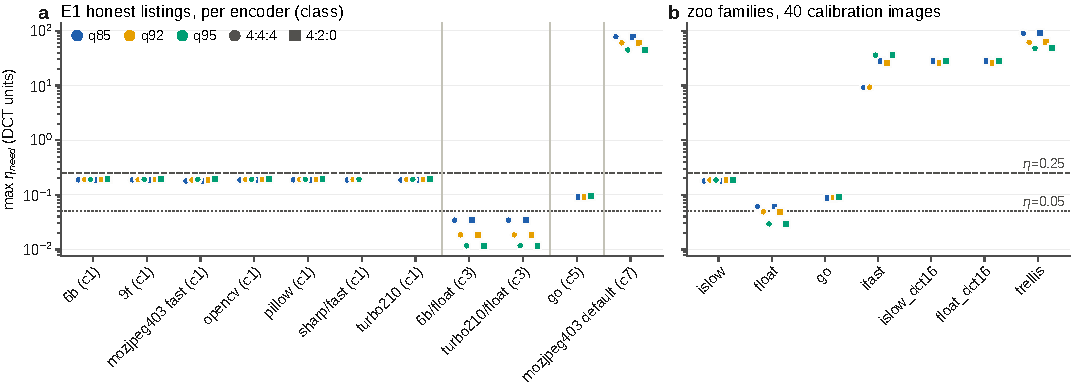
\includegraphics[width=\textwidth]{figs/fig4.pdf}
\caption{\textbf{E1: honest deviation per encoder and class} against the cell half-width. (a) largest $\eta_{\mathrm{need}}$ per
encoder, quality and sampling over the held-out listings; (b) encoder families on 40 calibration images, including the
non-members \texttt{ifast}, DCT-scaled chroma and trellis.}
\label{fig:e1}
\end{figure}

\begin{figure}[!htbp]
\centering
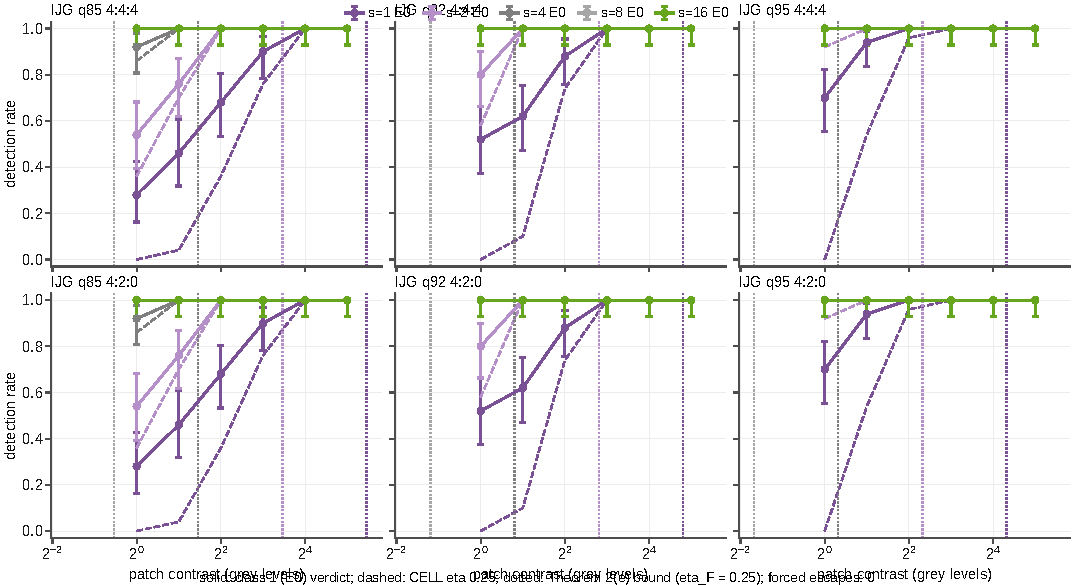
\includegraphics[width=0.9\textwidth]{figs/fig5.pdf}
\caption{\textbf{E2: detection of an $s\times s$ constant patch} against its contrast, per upload profile (9,000 listings).
Solid: \Ezero{}; dashed: the tolerant cell at $\eta=0.25$; dotted: the Theorem~\mainref{thm:cell}(e) forced-rejection
bound. No forced escape was observed.}
\label{fig:e2}
\end{figure}

\begin{figure}[!htbp]
\centering
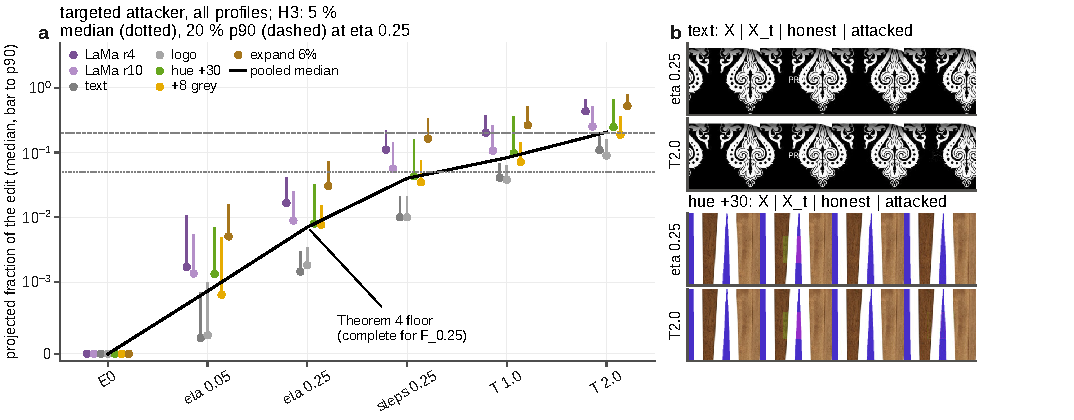
\includegraphics[width=0.92\textwidth]{figs/fig6.pdf}
\caption{\textbf{E3: projected fraction of an edit that reaches the screen} under an optimal attacker, from \Ezero{} (zero by
construction) through the tolerant cells to fixed pixel thresholds; the Theorem~\mainref{thm:minimality} floor for any
verifier complete for $\mathcal{F}_{0.25}$.}
\label{fig:e3}
\end{figure}

\begin{figure}[!htbp]
\centering
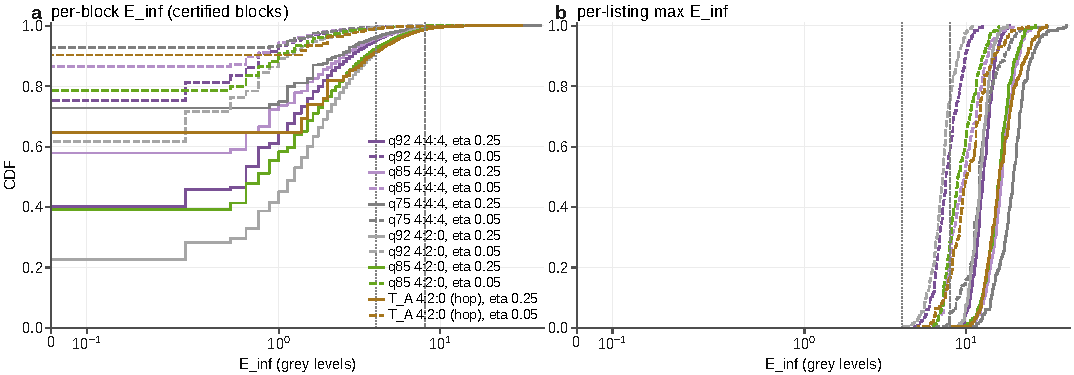
\includegraphics[width=0.9\textwidth]{figs/fig7.pdf}
\caption{\textbf{E3: per-block and per-listing $\Einf$ distributions} for the tolerant classes.}
\label{fig:einf}
\end{figure}

\textbf{Further E2/E3 numbers.} The six E2 upload profiles are q85, q92 and q95 at 4:4:4 and 4:2:0. In E3 the tolerant
cell is below the former pixel threshold $T=2.0$ in every class (one-sided Wilcoxon, Holm-adjusted $p<10^{-190}$), and a
table-grinding attacker realises a median 0.45\% (90th percentile 2.3\%, $n=97$) of the edit at $\eta=0.25$.

\section{Baselines (E4)}
\label{sec:e4}
\label{sec:detection}
Table~\ref{tab:e4} is the full E4 table (both profiles, every baseline and $\Delta$, the A10 result); the main text
prints a condensed version. Table~\ref{tab:b5} gives the per-pixel tolerant comparator E19 on the same items; its
protocol and the \Eone{}-cell comparator E21 are described in \S\ref{sec:x1}.
\begin{table}[!t]
\centering
\caption{E4 detection at a calibrated FPR of 1\%. TPR (\%) per attack class; FRR (\%) on the honest
test listings. A3sd, A6sd and A7sd have 50 attacks each, so their rates are whole percent.}
\label{tab:e4}
\fontsize{7}{8}\selectfont\setlength{\tabcolsep}{1.3pt}
\begin{tabular*}{\columnwidth}{@{\extracolsep{\fill}}lrrrrrrrrrr@{}}
\toprule
Method & A1 & A2 & A3 & A4 & A5 & A6 & A3sd & A6sd & A7sd & FRR\\
\midrule
\multicolumn{11}{@{}l}{\textit{Profile U85 (seller upload, q85)}}\\
\textbf{\sys{} \tierX{} (\Ezero{})} & 100.0 & 100.0 & 100.0 & 100.0 & 100.0 & 100.0 & 100 & 100 & 100 & 0.0\\
\hspace{4pt}\tierT{} (4:4:4 table) & 86.9 & 91.9 & 100.0 & 68.7 & 91.9 & 89.9 & -- & -- & -- & 1.0\\
Sun--He--Tian $\Delta$=4 & 67.4 & 79.8 & 100.0 & 61.2 & 80.8 & 73.7 & 92 & 0 & 96 & 0.0\\
Sun--He--Tian $\Delta$=8 & 62.8 & 73.7 & 100.0 & 57.1 & 73.7 & 58.6 & 90 & 0 & 96 & 0.0\\
Sun--He--Tian $\Delta$=16 & 50.0 & 62.6 & 99.0 & 51.0 & 48.5 & 42.4 & 74 & 0 & 92 & 0.0\\
Signed thumbnail & 61.6 & 73.7 & 100.0 & 60.2 & 78.8 & 67.7 & 94 & 100 & 96 & 0.0\\
pHash & 0.0 & 1.0 & 2.0 & 15.3 & 0.0 & 0.0 & 0 & 38 & 2 & 0.3\\
PDQ & 0.0 & 2.0 & 13.1 & 24.5 & 0.0 & 0.0 & 2 & 78 & 10 & 0.0\\
Birthmark replay & 7.0 & 3.0 & 23.2 & 32.7 & 2.0 & 14.1 & 14 & 90 & 40 & 0.0\\
PROVES-style & 0.0 & 0.0 & 1.0 & 6.1 & 0.0 & 0.0 & 0 & 0 & 0 & 0.0\\
TruFor & 0.0 & 0.0 & 0.0 & 0.0 & 0.0 & 0.0 & 0 & 0 & 0 & 0.3\\
Mesorch & 0.0 & 0.0 & 0.0 & 0.0 & 0.0 & 0.0 & 0 & 0 & 0 & 0.0\\
TrustMark & 0$^{b}$ & 0$^{b}$ & 0$^{b}$ & 0$^{b}$ & 0$^{b}$ & 0$^{b}$ & 0$^{b}$ & 0$^{b}$ & 0$^{b}$ & 0.0\\
\midrule
\multicolumn{11}{@{}l}{\textit{Profile AMZ (after the P-AMZ re-encode)}}\\
\textbf{\sys{} \tierX{} (\Ezero{})} & 100.0 & 100.0 & 100.0 & 100.0 & 100.0 & 100.0 & 100 & 100 & 100 & 0.0\\
Sun--He--Tian $\Delta$=4 & 28.7 & 59.0 & 97.0 & 55.6 & 34.0 & 36.0 & 90 & 0 & 96 & 0.0\\
Sun--He--Tian $\Delta$=8 & 29.9 & 63.0 & 97.0 & 56.6 & 33.0 & 36.0 & 94 & 0 & 96 & 0.0\\
Sun--He--Tian $\Delta$=16 & 23.0 & 52.0 & 95.0 & 51.5 & 22.0 & 24.0 & 88 & 0 & 96 & 0.0\\
Signed thumbnail & 18.4 & 39.0 & 90.0 & 55.6 & 20.0 & 16.0 & 82 & 100 & 92 & 0.3\\
pHash & 0.0 & 0.0 & 1.0 & 15.2 & 0.0 & 0.0 & 0 & 42 & 4 & 0.0\\
PDQ & 0.0 & 0.0 & 1.0 & 28.3 & 0.0 & 1.0 & 0 & 80 & 10 & 0.0\\
Birthmark replay & 0.0 & 0.0 & 2.0 & 37.4 & 0.0 & 2.0 & 8 & 70 & 42 & 0.0\\
PROVES-style & 0.0 & 0.0 & 0.0 & 7.1 & 0.0 & 0.0 & 0 & 0 & 0 & 0.0\\
TruFor & 4.6 & 4.0 & 4.0 & 2.0 & 4.0 & 4.0 & 0 & 0 & 0 & 3.0\\
TrustMark & 0$^{b}$ & 0$^{b}$ & 0$^{b}$ & 0$^{b}$ & 0$^{b}$ & 0$^{b}$ & 0$^{b}$ & 0$^{b}$ & 0$^{b}$ & 0.0\\
\bottomrule
\end{tabular*}
\tabnote{\fontsize{7}{8}\selectfont $^{b}$ by design (TrustMark is a soft binding and does not localise edits). A10 is scored for \tierT{} only: median projected fraction 0.80 under the \tierTa{} table (\Ezero{}: 0). No baseline dominates \sys{} in any cell (exact McNemar, Holm $p<0.05$). Not shown: CAT-Net, EditGuard and OmniGuard (gate failed: published numbers only, see \S\ref{sec:e4}); Mesorch at AMZ (run at U85 only); \tierT{} at AMZ (\tierT{} is unlinked through platform hops in the evaluated design). A6sd: tier-test verdict; the pixels added outside the drawn silhouette are reported separately and never scored as detection.}
\end{table}
\begin{table}[!t]
\centering
\caption{E19: per-pixel tolerant comparator. TPR (\%) at FPR 1\% of the per-pixel tolerant scores on the E4 test items, with the calibrated threshold
$\theta$ (grey levels) and the honest test false positives (FP, out of 299). \sys{} \tierX{} is 100.0 on every cell with 0/299 honest. Bold:
not significantly below \sys{} (exact McNemar $p\ge0.05$).}
\label{tab:b5}
\fontsize{7}{8}\selectfont\setlength{\tabcolsep}{1.2pt}
\begin{tabular*}{\columnwidth}{@{\extracolsep{\fill}}lrrrrrrrrrrr@{}}
\toprule
Score & $\theta$ & A1 & A2 & A3 & A4 & A5 & A6 & A3sd & A6sd & A7sd & FP\\
\midrule
\multicolumn{12}{@{}l}{\textit{Profile U85}}\\
\texttt{pix\_max} & 91 & 27.9 & 42.4 & 89.9 & 11.2 & 0.0 & 4.0 & 30 & \textbf{96} & 54 & 0\\
\texttt{pix\_max\_sil} & 91 & 27.9 & 42.4 & 89.9 & 11.2 & 0.0 & 4.0 & 30 & 8 & 54 & 0\\
\texttt{blk\_mean} & 9.51 & 52.3 & 67.7 & \textbf{100.0} & 45.9 & 6.1 & 53.5 & 70 & \textbf{100} & 82 & 1\\
\texttt{blk\_mean\_sil} & 9.28 & 54.7 & 67.7 & \textbf{100.0} & 45.9 & 7.1 & 53.5 & 74 & 4 & 86 & 1\\
\midrule
\multicolumn{12}{@{}l}{\textit{Profile AMZ}}\\
\texttt{pix\_max} & 148 & 3.4 & 7.0 & 7.0 & 7.1 & 0.0 & 0.0 & 24 & 62 & 36 & 0\\
\texttt{pix\_max\_sil} & 139 & 3.4 & 9.0 & 11.0 & 9.1 & 0.0 & 0.0 & 24 & 0 & 40 & 0\\
\texttt{blk\_mean} & 18.15 & 11.5 & 37.0 & \textbf{100.0} & 32.3 & 0.0 & 8.0 & 58 & \textbf{100} & 76 & 3\\
\texttt{blk\_mean\_sil} & 18.15 & 11.5 & 37.0 & \textbf{100.0} & 32.3 & 0.0 & 8.0 & 58 & 2 & 76 & 0\\
\bottomrule
\end{tabular*}
\end{table}

\textbf{Published-numbers rows.} EditGuard and OmniGuard were not run because their repositories grant no licence;
CAT-Net~\cite{kwon2022learning} passed its licence gate but its weights could not be downloaded (every download from
the official folder was refused). These methods are listed in the note of Table~\ref{tab:e4} instead of as rows; the published numbers we
rely on are those quoted in Sec.~\mainref{sec:related} (e.g., an off-the-shelf CAT-Net F1 of 0.02 on fully regenerated
inpainting~\cite{mareen2026tgif2}).

\textbf{Further E4 numbers.} Null edits (no pixel changed) were excluded and reported (41 listings), and 72 attacked
items were skipped because no textured point lay inside the silhouette and the certified region. TrustMark's clean
decode on the honest test listings is 298/299 (U85), 297/299 (AMZ) and 299/299 (P-SHOP); after the frozen removal
attacker it is 201/299, 215/299 and 209/299. Mesorch at FPR~5\% (threshold 0.9999982, honest FRR 7.4\%) detects A1 4.7\%,
A2 6.1\%, A3 2.0\%, A4 7.1\%, A5 6.1\%, A6 7.1\%, A3sd 6.0\%, A6sd 4.0\% and A7sd 4.0\%. TruFor ran on 2,696 images
with a measured peak of 4,361~MB; its honest FRR at AMZ is 3.0\% at the FPR-1\% threshold (a calibration/test shift). The 150 diffusion attacks took a median of 116.5~s each (peak 6,338~MB).

\begin{table}[!htbp]
\centering\tabsize
\caption{\textbf{A10: threshold-hugging edits.} Median (90th percentile) projected fraction of a targeted edit that passes \tierT{} (table f1 4:4:4),
against the \Eone{} cell at $\eta=0.25$ (E3, q85 4:4:4); \Ezero{} passes 0. $n=100$ per edit.}
\label{tab:a10}
\begin{tabular}{@{}lrrr@{}}
\toprule
Edit & \tierT{} median (p90) & accepted & \Eone{}, $\eta=0.25$ (median) \\
\midrule
brighten 8, 32 px & 0.308 (0.427) & 100/100 & 0.007 \\
expand 6\%, $R=40$ & 0.796 (0.943) & 100/100 & 0.031 \\
LaMa removal $r=10$ & 0.413 (0.762) & 100/100 & 0.009 \\
LaMa removal $r=4$ & 0.771 (0.900) & 100/100 & 0.017 \\
logo 24 px, $\alpha=0.6$ & 0.146 (0.194) & 100/100 & 0.002 \\
recolour hue 30, 48 px & 0.431 (0.724) & 98/100 & 0.007 \\
text 12 px & 0.107 (0.218) & 100/100 & 0.001 \\
\bottomrule
\end{tabular}
\end{table}
LaMa denotes the inpainting model of~\cite{suvorov2022resolutionrobust}.

\textbf{Tier-T test FRR per profile.} f0 4:2:0, f0 4:4:4, f1 4:2:0, f2, f3 and f4 (both samplings): 0/299 each;
f1 4:4:4: 3/299 = 1.003\% (95\% CP interval [0.0021, 0.0290]). The order-statistic guarantee is
$P(\text{FRR}>1\%)\le0.0495$ per profile, so one profile in ten above 1\% is within its reach, but the registered
point prediction fails for that profile.

\textbf{A6sd and the honest coverage check.} The A6sd tier-test column was predicted to stay below 100\% (the ring
touches only boundary blocks), but \sys{} detected 50/50 on both profiles; the likely mechanism, not diagnosed per
listing, is that the ring meets certified MCUs because $A$ is dilated beyond $\Sil$. The registered honest \tierT{}
coverage check (every honest 256-px listing tests at least one block) fails as written on 1/299: every existing listing
tests at least one block (minima 618 and 594 on the two kernels), but one thin product has no 256-px listing at all (refused below
the upload floor). The rule that a claim certifying nothing is \G{0} is unchanged.

\section{Residual surface and tolerant comparators (E13, E19, E21)}
\label{sec:e13}
\label{sec:x1}
\label{sec:additional}
The additional experiments were registered after the main results (E1--E12), each before its own run or analysis
(registration record: \S\ref{sec:disclosure}). E13--E17 were registered together, with their predictions, before any run on test
masters; E17b and E18--E21 were registered individually afterwards. Table~\ref{tab:xpred} quotes every registered prediction with its outcome; the E19 and E21
predictions quote the registration's own rule for what the paper may claim. E13 measures how far a white-box seller who
stays inside the admissible programs can change the displayed product while keeping \G{3} or \G{4}, starting from the
honest \G{4} constant-white listing of each E5 test master (Fig.~\ref{fig:x1}). In its tone row, the cosmetics
category cap makes a tone table whose product p95 $\Delta E_{00}$ exceeds 2.0 major (\G{2}) for cosmetics and apparel
listings, so only the minor class remains.
\begin{table*}[!t]
\centering\fontsize{7}{8.1}\selectfont
\caption{Additional experiments: registered predictions and outcomes. Predictions are quoted from the registration
without implementation names. E13--E17: registered together; E17b (in the E17 row) and E18--E21: each registered
before its own run or analysis; ``descriptive'': the prediction holds by construction or only describes a rate.}
\label{tab:xpred}
\renewcommand{\arraystretch}{1.0}\setlength{\tabcolsep}{4pt}
\begin{tabularx}{\textwidth}{@{}L{1.25cm}YL{6.5cm}@{}}
\toprule
ID & Registered prediction & Outcome \\
\midrule
E13 tone & A monotone tone table can hold the product's p95 $\Delta E_{00}$ just under the class thresholds while raising the mean / p99 product $\Delta E_{00}$ well above a just-noticeable difference ($\Delta E_{00}>1$--2), at \G{4} for the minor class and \G{3} for the moderate class; the cosmetics category cap (p95 $\le2.0$) limits it to the minor level. & Holds: mean 1.64 (\G{4}), 3.35 (\G{3}); targeted p99 3.16 / 7.03; 100/100 each; cosmetics mean-objective \G{4} on 88/100 (targeted \G{3} on 94/100). \\
E13 $D$ & With $k=\lfloor|\Mcert|/51\rfloor$, a declared-retouch blob or boundary trim reaches \G{3} (not \G{2}) while removing or replacing a visible product part; the trim changes the visible shape (IoU $<1$, Hausdorff $>0$) and the removed part is drawn as a hole; $k+1$ drops to \G{2}. & Holds: blob \G{3} 100/100 (2.95\% replaced); trim \G{3} 99/100 (IoU 0.973, Hausdorff 54~px; one \G{4} from a capture miss); $k+1$ \G{2} 100/100. \\
E13 gen. & Generated content placed strictly in uncertified MCUs beyond the certified footprint is never scored by the \tierXa{} test (0 generated pixels in the certified set and in $\Sil$); the listing keeps a positive level (\G{3}, background generated-declared) and is not detected. Reported as a residual, not a defect. & Descriptive (true by construction): 0 generated pixels in $\Mcert$ and $\Sil$; \G{3} 30/30 (also with a declared bridge $D$), i.e., not detected. Adversarial-scene arm not run. \\
E14 & The median miss is 0 in every stratum; a minority have a material capture miss ($>2\%$), with a per-stratum CP upper bound that we report. & Descriptive: median 0; $>2\%$ on 20, 8, 4 of 100 (bounds 0.277, 0.140, 0.089). \\
E15 & Honest star failures $=0$ on every profile; the \WF{3} star ladders are at the source level on 100\% of in-scope honest renditions; every attack case matches its expected (linked, error, level). & Holds: 0 failures (3,603 renditions); 185/185; 38/38. All masters ABO. \\
E17 & The 12 rows reproduce on Besu up to calldata-byte and ECDSA-$v$ differences; if Besu cannot run them, they are marked EDR-only with the reason. & Partly: 11/12; the 65,535-MCU proof is EDR-only (transaction size). E17b: mined with the pool limit raised ($-60$ gas). \\
E18 & \AS{9} is supported in its restricted form iff every decoder of the family (libjpeg-turbo and IJG 6b at \islow{} with fancy upsampling, Pillow and OpenCV as built) displays $\Dstar$ bit-exactly on the certified region of every sampled file; Part A (a re-check of the hashes that E9 recorded) passes iff every recorded hash equals the $\Dstar$ hash. & Holds: 3,600/3,600 pairs on 400 files; Part A 202/202 for Pillow, OpenCV and Chrome. Outside the family: \S\ref{sec:b1}. \\
E19 & Where \texttt{pix\_max} TPR is below \sys{} with McNemar $p<0.05$, the paper may say that a per-pixel tolerant test on the same openings misses edits the exact test catches; elsewhere it must say tolerance does not cost detection. & Below on 17/18 cells (U85 0.0--96.0\%, AMZ 0.0--62.0\%; unchanged under Holm's correction); not on A6sd at U85 (96.0\%, $p=0.5$). \\
E20 & The \G{2} renditions at $500\times375$ are mainly wide or tall products iff $\ge80\%$ of the \G{2} renditions at $500\times375$ lie outside an aspect band around 4:3 and the \G{2} share inside the band is materially lower; otherwise the dominant recorded cause replaces it. & Met literally (92.2\% outside; 58.8\% vs 100\%), wrong in substance: every \G{2} is \emph{partial} from the 4:3 crop, square canvases included (26/26). \\
E21 & Where the calibrated \Eone{}-cell TPR is below \sys{} with McNemar $p<0.05$, the paper may say that even the cell test on the same openings misses edits; elsewhere it must say that a per-cell tolerant test detects about as much and that the advantage is the zero excess and the one-point acceptance set. & Below on 0/18 cells: 100\% everywhere ($\eta=0.178$, 0.181), honest 1/299, 0/299; fixed $\eta=0.25$: 100\%, 0/299. \\
\bottomrule
\end{tabularx}
\end{table*}
\begin{figure*}[!t]
\centering
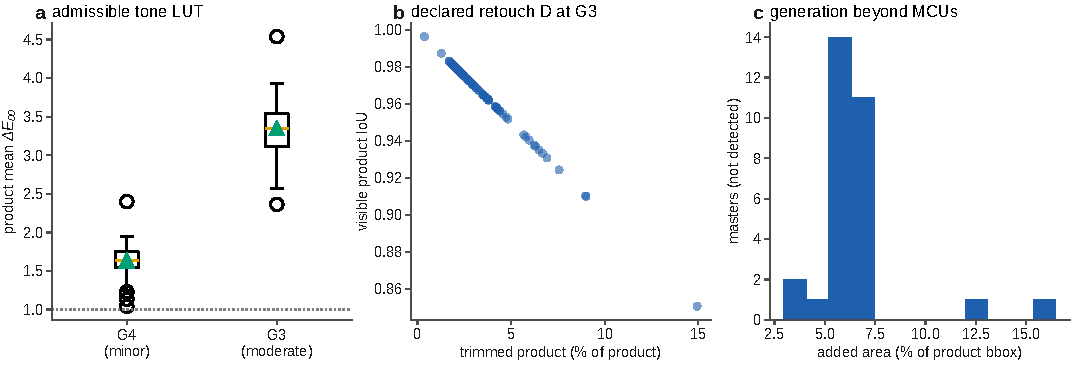
\includegraphics[width=\textwidth]{figs/fig_x1_residual.pdf}
\caption{\textbf{Residual surface of E13.} (a) Product mean $\Delta E_{00}$ reached by the mean-objective monotone tone table while
the tone class stays minor (\G{4}) or moderate (\G{3}); triangle: mean; dotted line: $\Delta E_{00}=1$. (b) Declared
retouch $D$ with $k=\lfloor|\Mcert|/51\rfloor$ MCUs used to trim the product boundary: visible product IoU against the
trimmed fraction (99 listings at \G{3}). (c) Diffusion content added wholly in uncertified MCUs beyond the certified
footprint (30 listings, all \G{3}, none detected): added area relative to the product's bounding box.}
\label{fig:x1}
\end{figure*}
The E19 table is Table~\ref{tab:b5} (\S\ref{sec:e4}).
\textbf{Tone (prediction holds).} A monotone $3\times256$ table searched over five families and 12 directions keeps
the tone class while moving the product: at \G{4} (minor) the median product mean $\Delta E_{00}$ is 1.64 (90th
percentile 1.86) with the mean objective, and the targeted 99th-percentile $\Delta E_{00}$ reaches 3.16; at \G{3}
(moderate) the mean is 3.35 (p90 3.83) and the targeted p99 7.03 (maximum 9.60); 100/100 listings stay at their level in
each case. Under the cosmetics cap the mean-objective table stays minor (\G{4}) on 88/100, and the targeted table
reaches \G{3} on 94/100 with p99 5.25. A \G{4} label prints no tone disclosure; \G{3} prints ``colour adjusted'' with
the $\Delta E_{00}$ statistics. The search gives lower bounds on a white-box optimum; the class bounds any table at
$\Delta E_{00}\le4$ (\G{4}) and $\le10$ (\G{3}) on certified product pixels.

\textbf{Declared retouch (prediction holds).} With $k=\lfloor|\Mcert|/51\rfloor$ declared MCUs (median $k=61$) a blob
recolour or inpaint stays \G{3} on 100/100 while replacing a median 2.95\% of the product pixels; a boundary trim stays
\G{3} on 99/100 with visible-product IoU 0.973 and Hausdorff distance 54~px (medians); with $k+1$ MCUs all 100 drop to
\G{2}. The printed evidence says ``retouched areas marked'', draws the $D$ MCUs as holes in $\Sil$ and prints the
retouched fraction. The one trim at \G{4} is a capture miss: no certified MCU of that master contains ground-truth
product pixels, so nothing was declared.

\textbf{Generation beyond the certified footprint (prediction holds; a residual).} Stable Diffusion 1.5 inpainting of
a region in uncertified MCUs beyond the footprint (30 masters) put 0 generated pixels into $\Mcert$ or $\Sil$; every
listing stayed \G{3} with ``background AI-generated'' (median gap to the product 13.4~px, about the dilation), also
with a declared bridge $D$ (median 64 MCUs; \G{3} 30/30). Such content is not detected: a buyer can only see that it
lies outside the drawn outline. The E4 A6sd ring, which meets certified MCUs, was detected 50/50.

\textbf{Not run.} Adversarial scene content against the capture segmenter (the fourth E13 arm) was removed from scope
during development; capture coverage loss is measured descriptively by E14 (\S\ref{sec:e5}).

\textbf{Reference-holding rows of E4 (post-registration analysis, disclosed).} After the E4 results were known, we
took its reference-holding tolerant tests, which rebuild the same declared-program reference from the openings and are
calibrated at matched FRR, as a first equal-information comparator; no new run. This is an extraction made with the
values known, not a rule fixed before any result, and these coarse features are not the strongest tolerant test on the
same openings, so the manuscript uses E19 instead. At FPR 1\% on U85, Sun--He--Tian detects 67.4--100 ($\Delta=4$),
57.1--100 ($\Delta=8$) and 42.4--99.0\% ($\Delta=16$) per class except A6sd (0\%), and the thumbnail 60.2--100\%; at AMZ
the tolerant tests fall to 16.0--97.0\% (A6sd and A7sd aside); \sys{} detects 100\% everywhere with 0/299 honest
convictions per profile (Table~\ref{tab:e4}).

\textbf{E19: global-threshold per-pixel comparator.} Its registration (committed in afd30d3 at 2026-10-07T23:48:06Z before the
run, with no score computed) fixes the scores, the calibration and the interpretation rule. The runner reuses the frozen
E4 items and data factory unchanged (masters, splits, attack draws, diffusion attacks, null-edit rule). For each
listing, $Z=\Dstar$ of the displayed bytes (the U85 upload, or the P-AMZ L1000 rendition for AMZ), $R$ the reference
\sys{} rebuilds from the openings (pushed through the declared hop with its exact kernel for AMZ) and $C$ the certified
pixels (pushed through the hop for AMZ). The primary score \texttt{pix\_max} is $\max_{p\in C,\,c}|Z-R|$, a pixel test
with one global threshold; \texttt{pix\_max\_sil} restricts it to $C\cap\Sil$; \texttt{blk\_mean} is the largest mean
$|Z-R|$ over the certified pixels of an $8\times8$ block of the displayed grid (blocks with $\ge32$ certified pixels);
\texttt{blk\_mean\_sil} is its $\Sil$ version. The FPR-1\% threshold is the maximum over the 299 honest calibration
listings per profile; a test item is flagged iff its score exceeds it. \sys{} is the frozen \tierXa{} verdict of the E4 run
on the same item keys; the paired test is an exact two-sided McNemar test. 2,696 items were scored (0 errors); 6 were
skipped (no listing or no textured point) and 28 null edits excluded, as in E4. Table~\ref{tab:b5} gives the result.
By the registered rule, \texttt{pix\_max} is significantly below \sys{} on 17 of 18 (class, profile) cells; Holm's
correction over the 18 cells changes no decision (the largest significant $p$, 0.002, is below its Holm threshold
0.025). On A6sd at U85 (48/50, $p=0.5$) the difference is not significant. The best variant, \texttt{blk\_mean}, ties
\sys{} ($p\ge0.05$) only on A3 and A6sd on both profiles, at an honest test FPR of 1/299 (U85) and 3/299 (AMZ). The
$\Sil$ variants lose A6sd because the ring lies outside $\Sil$.

\textbf{E21: the \Eone{} cell as an equal-information comparator.} Registered in 076b16d (2026-10-08T00:55:43Z) before
the run, on the same 2,696 E4 items. The score is the smallest slack that accepts every tested coefficient,
$\eta_{\mathrm{need}}=\max_k(|c_kQ_k-F_k|-Q_k/2)$ in DCT units, where $F$ is the DCT of the reference front end, over
the blocks of $\Mcert$ at U85 and, at AMZ, over the rendition MCUs that contain a pushed certified pixel, against the
hop reference that a verifier rebuilds from the openings ($\Dstar$ of the exact upload, resized by the declared hop).
Thresholds are the calibration maxima (FPR 1\%): $\eta=0.178$ (U85) and 0.181 (AMZ). The cell test detects 100\% of
every class on both profiles (McNemar $p=1$ against \sys{} on all 18 cells; against \texttt{pix\_max} $p\le0.002$ on
17 cells, $p=0.5$ on A6sd at U85) with 1/299 (U85) and 0/299 (AMZ) honest test alarms. Every attacked listing needs
$\eta_{\mathrm{need}}\ge1.0$ (U85; 1.026 at AMZ), every honest test listing at most 0.183, so the result does not
depend on where in $[0.18,1)$ the threshold lies; the design's fixed $\eta=0.25$ also detects 100\% with 0/299 honest
alarms, and $\eta=0.05$ rejects every honest listing. Against the reference of E19 at AMZ (the original pushed through
the hop, without the upload's quantisation) the cell test is weaker (48--100\%; descriptive), so the
transcoding-aware reference matters. By the registered rule, a well-designed per-cell tolerant test detects as much as
\sys{} on these attacks; \sys{}'s advantage over it is the zero adversarial excess (E3) and a one-point acceptance set with no
slack parameter (the fixed $\eta=0.25$ is also uncalibrated, but admits a whole cell), not the detection rate.

\section{Region coverage (E5, E14)}
\label{sec:e5}
\begin{figure}[!htbp]
\centering
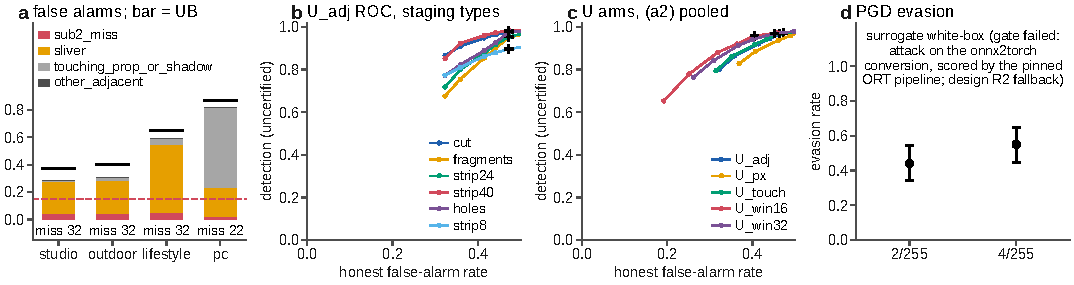
\includegraphics[width=\textwidth]{figs/fig9_e5.pdf}
\caption{\textbf{E5 region coverage} (H5; main Sec.~\mainref{sec:eval-e5}). (a) False alarms of $U>\tauU$ per honest workflow type, split by mechanical cause (sub-2\% capture
miss, sliver, touching prop or shadow, other adjacent); the black bar is the one-sided upper bound used by (a1), the
dashed line the 15\% criterion. (b) ROC of $U$ per mask-only staging type (detection among uncertified staged
listings against the honest false-alarm rate, $\tau\in\{8,\dots,128\}$; $+$ marks $\tauU=32$). (c) The same for the
registered $U$ variants, pooled over the (a2) types. (d) Surrogate white-box PGD evasion at $\epsilon=2/255$ and
$4/255$ with 95\% CP intervals.}
\label{fig:e5}
\end{figure}
\begin{table}[!htbp]
\centering\tabsize
\caption{\textbf{E5 per stratum.} $k/n$ per honest workflow type (false alarms of $U>\tauU$, with the one-sided 95\%
upper bound) and per mask-only staging type (detections, with the lower bound); last row: captures re-drawn by the
ground-truth reshoot rule.}
\label{tab:e5strata}
\begin{tabular}{@{}lrrr@{}}
\toprule
Measure & White & Scene & DIS \\
\midrule
Studio, false alarms (UB) & 16/80 (0.288) & 33/92 (0.449) & 28/96 (0.377) \\
Outdoor, false alarms (UB) & 17/80 (0.302) & 31/92 (0.427) & 35/96 (0.453) \\
Lifestyle, false alarms (UB) & 39/80 (0.585) & 53/92 (0.663) & 66/96 (0.765) \\
Product-conditioned (pc), false alarms (UB) & 47/51 (0.973) & 51/64 (0.875) & 48/63 (0.847) \\
\addlinespace[2pt]
Cut, detected (LB) & 1090/1096 (0.989) & 996/1014 (0.974) & 985/1038 (0.936) \\
Fragments, detected (LB) & 394/398 (0.977) & 455/473 (0.944) & 724/781 (0.910) \\
24-px strips, detected (LB) & 365/368 (0.979) & 600/626 (0.943) & 733/783 (0.920) \\
40-px strips, detected (LB) & 1099/1101 (0.994) & 1082/1097 (0.979) & 1060/1092 (0.961) \\
Holes, detected (LB) & 521/528 (0.975) & 279/290 (0.938) & 135/138 (0.945) \\
\addlinespace[2pt]
Ground-truth reshoots & 20/100 & 8/100 & 4/100 \\
\bottomrule
\end{tabular}
\end{table}
\textbf{Reported types.} Detached completion 95/100 (CP lower bound 0.898), detached twin 33/77 (0.333), low contrast
43/49 (0.773), occluder 47/50 (0.852), prop 48/48 (0.939), 8-px strips 373/416 (0.869). At $\tauU=32$ the registered
$U$ variants detect / falsely alarm: $U_{\mathrm{adj}}$ 10,891/11,239 and 478/1,298; $U_{\mathrm{px}}$ 11,003 and 525;
$U_{\mathrm{touch}}$ 10,876 and 470; $U_{\mathrm{win16}}$ 10,734 and 411; $U_{\mathrm{win32}}$ 10,869 and 458. Design
effects (Kish): studio $\hat\rho=0.273$, deff 2.56; outdoor 0.381, 3.17; lifestyle 0.109, 1.38. The mask-reuse check
flipped 2/99 $U$ decisions (contingency at 5\% not triggered), and two independent runs produced byte-equal public masks on
50/50 listings. Under the surrogate PGD at $\epsilon=4/255$, evasion per staging type is cut 15/28, fragments 6/14,
holes 6/9, 24-px strips 10/16, 40-px strips 17/30 and 8-px strips 1/3. The evaluation's ground-truth reshoot rule (more
than 2\% of the product missed) fired with U\textsuperscript{2}-Netp~\cite{qin2020u2net} as capture model on 13/17 DIS
capture attempts (miss median 0.287) and with BiRefNet-lite on 4/117 (DIS), 9/119 (scene) and 21/114 (white) capture
attempts, i.e.\ 4, 8 and 20 of the 100 accepted masters
per stratum (Table~\ref{tab:e5strata} counts per accepted master). The (a1) denominators exclude the listings of these 32
masters (pasted types) and 22 incomplete pc listings. BiRefNet-lite as the public (listing-side) segmenter does not help: 195/268 false
alarms.

\textbf{Hand audits (protocol).} Two registered audits are reported as agreement only and change no mechanical label
(results: \S\ref{sec:handaudit}). Audit~1 covers the 30 honest false-alarm listings that come first by a fixed hash of the
listing key (domain string \path{CUTLINE-E5-causeaudit-v1}; \path{cause_audit_keys} in \path{experiments/s9/e5/e5.json}),
as 145 units (97 numbered components and 48 residual groups). Audit~2 covers the 30 masters of the ground-truth
contact sheet (\path{experiments/s9/e5m/audit_sheet.jpg}). Before rendering, the components and causes were recomputed
with the unchanged code path and checked against \path{e5_honest.jsonl}. The rendered items, the unit definitions and
the answer categories are in \path{experiments/s9/hand_audit/} (\path{manifest.json}, \path{README.md}, regenerated by
\path{build_hand_audit.py}). Five annotators labelled each audit jointly on the labelling page
(\path{audit_page.html}) and agreed on one consensus label per unit or image. The mechanical label or the rule's
verdict was shown beside the choices. The labels were exported on 2026-10-11 to \path{labels_audit1.json} and
\path{labels_audit2.json}. They are scored by \path{score_hand_audit.py} (stdlib), whose rule was committed in
b660ce0 before any label existed, into \path{hand_audit_result.json}, which \path{experiments/s9/s9_exit.py} reads
for rows~3 and~5 of the S9 exit report. Because the labels are consensus labels, no inter-annotator agreement is
reported.

\textbf{E14: coverage against ground truth.} For the BiRefNet-lite capture of each E5 test master (100 per stratum),
the fraction of ground-truth product pixels outside $\Sil$ equals that outside $A$ for every master (the whole-frame
listing certifies the placed region exactly). Its median is 0 in every stratum; its mean is 4.7\% (white; 95\% CI
2.2--7.7\%), 4.5\% (scene; 1.4--8.4\%) and 0.39\% (DIS; 0.14--0.75\%), 3.2\% over all 300. More than 2\% is missed on
20/100 (white, CP upper bound 0.277), 8/100 (scene, 0.140) and 4/100 (DIS, 0.089), 32/300 overall (0.141): exactly the
masters that the evaluation's ground-truth reshoot rule re-drew. A deployed app has no ground truth, so these misses
remain an operational residual. The registered prediction (median 0, a minority with a material miss) holds; this
is the first ground-truth measurement of how often \AS{7} fails.

\begin{table}[!htbp]
\centering\tabsize
\caption{\textbf{Workflow families \WF{1}--\WF{3}.} Share of honest listings at the target level, $U$ printed only (the setting
in force after gate E5 failed) and $U$ as a level criterion (as first computed); 95\% CP intervals. \WF{1} and \WF{2}
pass; \WF{3} is deployable on one-hop (star) ladders only: every cascade row straddles 0.5 and the E6 P-SHOP cascade rows
are below it (bounded 0.481; off/on 50/103 = 0.485, [0.386, 0.586]).}
\label{tab:gw}
\begin{tabular}{@{}llllll@{}}
\toprule
Family & fill & capture & target & $U$ printed only & $U$ a criterion \\
\midrule
\WF{1} constant & bounded & BiRefNet-lite & \G{4} & 300/300 [0.988, 1.000] & 288/300 \\
\WF{1} constant & bounded & U\textsuperscript{2}-Netp & \G{4} & 50/50 [0.929, 1.000] & 50/50 \\
\WF{1} constant & off / on & BiRefNet-lite & \G{4} & 100/100, 100/100 & 96/100, 99/100 \\
\WF{1} constant (halo-free variant) & bounded & BiRefNet-lite & \G{4} & 50/50 & 46/50 \\
\WF{2} lifestyle+pc & bounded & BiRefNet-lite & \G{3} & 500/500 [0.993, 1.000] & 150/500 [0.260, 0.342] \\
\WF{2} lifestyle+pc & bounded & U\textsuperscript{2}-Netp & \G{3} & 89/89 & 25/89 \\
\WF{2} lifestyle+pc & off / on & BiRefNet-lite & \G{3} & 168/168, 168/168 & 46/168, 49/168 \\
\WF{2} lifestyle+pc (halo-free variant) & bounded & BiRefNet-lite & \G{3} & 89/89 & 23/89 \\
\midrule
\multicolumn{6}{l}{\WF{3} (share at the source listing's level; \WF{2} and halo-free sources through P-AMZ / P-SHOP), $U$ printed only:} \\
\multicolumn{6}{l}{\quad star 440/440, 447/447; cascade 150/290 = 0.517 [0.458, 0.576], 150/297 = 0.505 [0.447, 0.563]} \\
\multicolumn{6}{l}{\quad $U$ a criterion (as first reported): star 440/440, 447/447; cascade 250/290, 255/297} \\
\multicolumn{6}{l}{\WF{3} of \WF{1} (E6 ladders, bounded fill), $U$ printed only: star 895/895, 918/918;} \\
\multicolumn{6}{l}{\quad cascade P-AMZ 299/596 = 0.502 [0.461, 0.543], P-SHOP 298/619 = \textbf{0.481} [0.441, 0.522]} \\
\bottomrule
\end{tabular}
\end{table}

\section{E5 hand audits}
\label{sec:handaudit}
The E5 registration includes two hand audits, reported as agreement only; neither changes a mechanical label or
a decision. Audit~1 covers the 30 honest false-alarm listings that come first in the order of
$H(d\,\|\,\mathit{key})$ with domain string $d=$ \path{CUTLINE-E5-causeaudit-v1}. Audit~2 covers the 30 accepted
masters of the ground-truth contact sheet (15 white, 15 scene, drawn by $H(d'\,\|\,\mathit{id})$ with
$d'=$ \path{CUTLINE-E5-audit-v1}). The scoring rule
was committed before any label existed (commit b660ce0, 2026-10-07 20:45:36 UTC).
\emph{Protocol.} Five annotators labelled each audit jointly by eye, from rendered overlays and zoom crops and without
re-running any rule, and reached one consensus label per unit (audit~1) or image (audit~2); the labels are therefore
not independent, and no inter-annotator agreement is reported. The mechanical label (audit~1) or the rule's verdict
(audit~2) was shown beside the answer choices, so the audits are not blind.
\emph{Units (audit~1).} The 30 listings have 3,410 $\Cadj$ components, most of 1--3~px. Each listing therefore shows
its largest components until they hold $\ge90\%$ of the $\Cadj$ pixels (at most 8), plus the largest component of each
mechanical cause not yet shown. All other components form one residual group per mechanical cause. This gives 145
units (97 components, 48 groups). Each unit receives one of the four causes or ``unclear''.
\emph{Statistics.} The registered unit is the listing for audit~1 and the image for audit~2. A listing agrees iff
every one of its units agrees, and ``unclear'' counts as a disagreement. Intervals are two-sided 95\%
Clopper--Pearson. Table~\ref{tab:handaudit} gives the results.

\begin{table}[!t]
\centering\fontsize{7}{8.1}\selectfont
\caption{E5 hand audits (consensus labels of five annotators).
Top: agreement statistics. Bottom: audit~1 confusion matrix, mechanical cause (rows) $\times$ consensus label (columns);
no unit was mechanically a sub-2\% miss.}
\label{tab:handaudit}
\renewcommand{\arraystretch}{1.0}\setlength{\tabcolsep}{3pt}
\begin{tabular*}{\columnwidth}{@{\extracolsep{\fill}}lrrr@{}}
\toprule
Statistic & $k/n$ & rate & 95\% CP \\
\midrule
\multicolumn{4}{@{}l}{\textit{Audit 1: false-alarm causes (30 listings, 145 units)}}\\
Listing agreement (primary) & 5/30 & 16.7\% & 5.6--34.7\% \\
Label-set agreement & 22/30 & 73.3\% & 54.1--87.7\% \\
Unit agreement & 95/145 & 65.5\% & 57.2--73.2\% \\
Unit agreement, ``unclear'' excluded & 95/113 & 84.1\% & 76.0--90.3\% \\
Pixel-weighted unit agreement & 689,113/765,008 px & 90.1\% & -- \\
Cohen's $\kappa$ (units) & -- & 0.49 & -- \\
\multicolumn{4}{@{}l}{\textit{Audit 2: ground-truth validity (30 masters; the rule accepted all 30)}}\\
Judged valid (primary) & 30/30 & 100\% & 88.4--100\% \\
\quad white / scene & 15/15, 15/15 & 100\% & 78.2--100\% \\
\bottomrule
\end{tabular*}

\vspace{4pt}
\begin{tabular*}{\columnwidth}{@{\extracolsep{\fill}}lrrrrrr@{}}
\toprule
Mechanical $\downarrow$ / human $\rightarrow$ & miss & sliver & touch. & other & unclear & total \\
\midrule
sliver & 0 & 35 & 0 & 0 & 9 & 44 \\
touching prop / shadow & 3 & 6 & 52 & 7 & 19 & 87 \\
other adjacent & 0 & 1 & 1 & 8 & 4 & 14 \\
\midrule
total & 3 & 42 & 53 & 15 & 32 & 145 \\
\bottomrule
\end{tabular*}
\end{table}

The listing statistic (5/30) is strict: most listings have several units, and one disagreeing or ``unclear'' unit
makes the listing disagree. The set of causes agrees in 22 listings, and the pixel-weighted agreement (90.1\%) exceeds
the unweighted one (65.5\%), so the disagreements lie mostly in small components; 32 of the 50 disagreeing units are
``unclear''. Three units that the rule calls touching props or shadows were read as product misses, consistent with
the capture misses measured in E14. The audit supports the cause shares, approximately so for small regions, and does
not change the mechanical counts. Audit~2 agrees with the frozen validity rule on every image (pilot reference: 38/40).

\section{Verified hops (E6, E15, E20)}
\label{sec:e6}
\begin{figure}[!htbp]
\centering
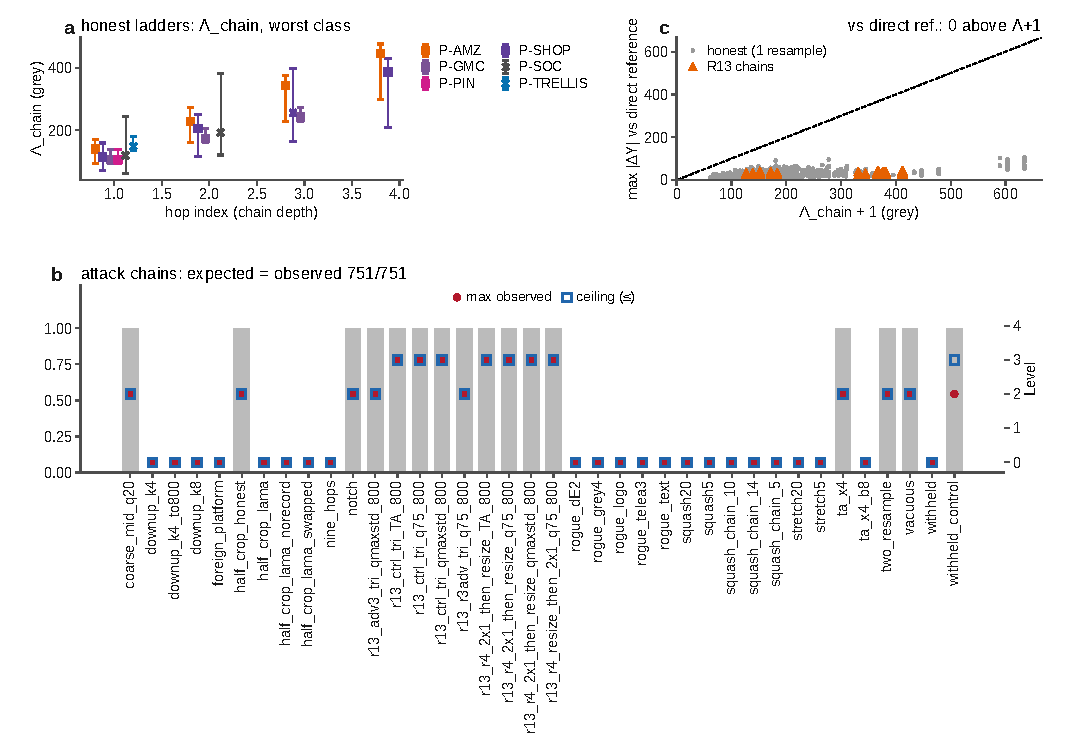
\includegraphics[width=0.92\textwidth]{figs/fig8_postfix.pdf}
\caption{\textbf{E6 verified hops after the three disclosed fixes} (the pre-registered version is Fig.~\ref{fig:e6-prereg}). (a)
$\Lchain$ and worst class along honest ladders per platform; (b) attack chains: share linked, maximum observed level
and the registered level ceiling, 751/751 renditions as predicted (case labels, e.g.\ \texttt{r13\_ctrl\_tri\_q75\_800}, are the artifact's case identifiers: control or adversarial chain, kernel, hop table, width); (c) maximum luma deviation from the direct reference
against $\Lchain+1$ on footprint-certified pixels.}
\label{fig:e6}
\end{figure}
\begin{figure}[!htbp]
\centering
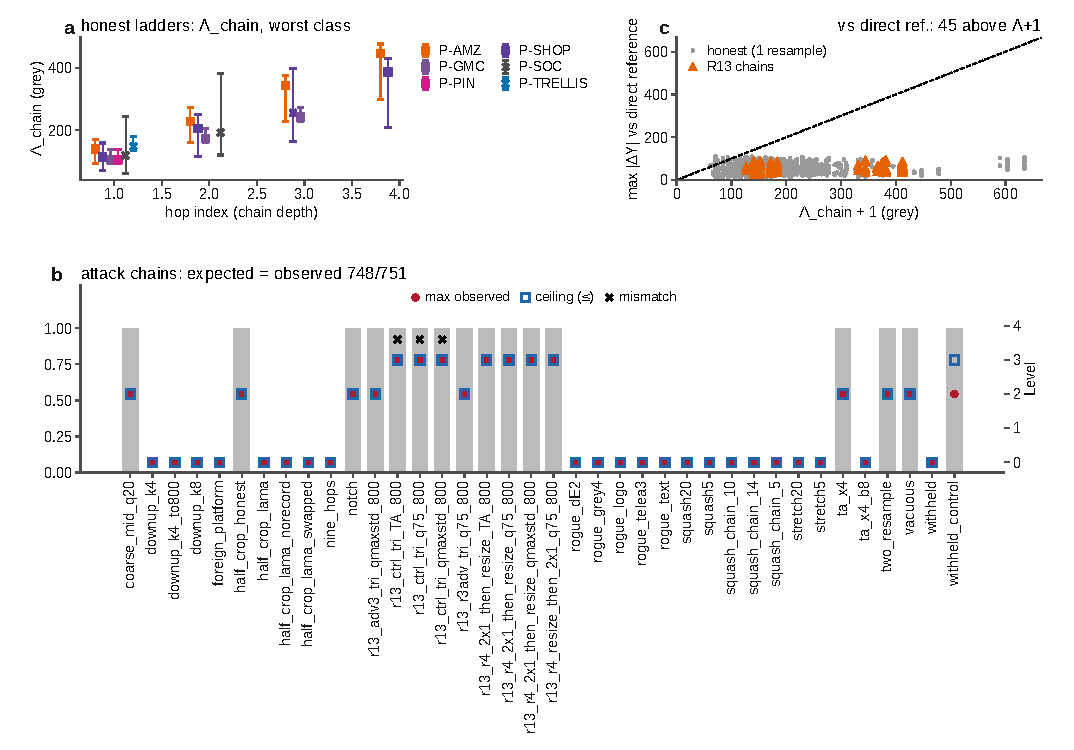
\includegraphics[width=\textwidth]{figs/fig8.pdf}
\caption{\textbf{E6 as pre-registered} (before the three disclosed fixes). Panels as in Fig.~\ref{fig:e6}. Panel (c)
counts 45 renditions above $\Lchain+1$: it excludes the one rendition with a rounded non-integer composed crop that the
46/8,603 of the text includes.}
\label{fig:e6-prereg}
\end{figure}
\begin{table}[!htbp]
\centering\tabsize
\caption{\textbf{E6 side by side.} Pre-registered run and the disclosed post-fix rerun (same criteria, one code digest).}
\label{tab:e6-side}
\begin{tabular}{@{}lrr@{}}
\toprule
E6 number & pre-registered & post-fix \\
\midrule
Honest in-scope renditions & 10,577 & 10,577 \\
Honest star failures (gate E6: must be 0) & \textbf{114} & \textbf{0} \\
\quad Go class 5 unlinked / $U$ flip up / $U$ flip down & 58 / 55 / 1 & 0 / 0 / 0 \\
Star per profile, failures: P-AMZ, P-GMC, P-GMC/go & 12, 11, 61 & 0, 0, 0 \\
\quad P-PIN, P-SHOP, P-SOC, P-TRELLIS & 2, 25, 3, 0 & 0, 0, 0, 0 \\
Go class 5 linked at $1000\times750$ & 28/86 & 86/86 \\
Attack cases as expected (gate E6: all) & \textbf{35/38} & \textbf{38/38} \\
Joint aspect maximum ($\le0.02$) & 0.015504 & 0.015504 \\
Tier-\cutid{X} share without cooperation (served) & 400/400 & 400/400 (reused) \\
Honest renditions above their source level & 69 & 0 \\
Renditions with $\le1$ resample measured & 8,603 & 8,661 \\
\quad luma above $\Lchain+1$, registered formula & 46 (max/$\Lchain$ 1.555) & 46 (1.555) \\
\quad luma above $\Lchain+1$, footprint-certified only & -- & 0 (max/$\Lchain$ 0.506) \\
\WF{3} star P-AMZ bounded / off / on & 888/895, 146/147, 147/147 & 895/895, 147/147, 147/147 \\
\WF{3} star P-SHOP bounded / off / on & 909/918, 151/153, 153/153 & 918/918, 153/153, 153/153 \\
\WF{3} cascade P-AMZ bounded / off / on & 361/596, 54/97, 50/97 & 363/596, 54/97, 50/97 \\
\WF{3} cascade P-SHOP bounded / off / on & 349/619, 55/103, 52/103 & 352/619, 56/103, 52/103 \\
P-TRELLIS own ceiling: \G{3} / \G{2} & 254 / 45 & 252 / 47 \\
\textbf{Gate E6} & \textbf{FAIL} & \textbf{pass (after three disclosed fixes)} \\
\midrule
\multicolumn{3}{l}{\emph{Re-derived from the same records with $U$ printed only (the setting in force after gate E5):}} \\
Honest star failures & \textbf{58} (P-GMC/go only) & 0 \\
Attack cases as expected & 38/38 & 38/38 \\
\WF{3} star P-AMZ / P-SHOP bounded & 895/895, 918/918 & 895/895, 918/918 \\
\WF{3} cascade P-AMZ bounded / off / on & 299/596, 50/97, 50/97 & 299/596, 50/97, 50/97 \\
\WF{3} cascade P-SHOP bounded / off / on & 298/619, 50/103, 50/103 & 298/619, 50/103, 50/103 \\
P-TRELLIS own ceiling: \G{3} / \G{2} & 299 / 0 & 299 / 0 \\
\textbf{Gate E6} & \textbf{FAIL} & \textbf{pass (after three disclosed fixes)} \\
\bottomrule
\end{tabular}
\end{table}
\textbf{E15: confirmatory rerun.} The post-fix code was rerun as a pre-registered confirmatory test on 50 masters never
used by any detection or level test (drawn by hash from the manifest ranks beyond the E1--E6 sets, which E12 had only
timed; all 50 are ABO, so Objectron and CO3D are not covered): 150 uploads, 1,460 items, 3,603 honest renditions.
Gate E6 passes: 0 honest star failures on P-AMZ ($n=678$), P-SHOP (687), P-GMC (273), P-GMC/go (123), P-SOC (100) and
P-PIN (50); 38/38 attack cases as expected; joint aspect maximum 0.0136 ($\le0.02$); Go class-5 renditions linked at
every size ($1000\times750$: 32/32); \WF{3} star renditions at the source level 185/185 (P-AMZ). Cascades keep the
source level for 0.37--0.39 (reported, no criterion).

\textbf{E20: why $500\times375$ renditions end at \G{2}.} Registered in afd30d3 (2026-10-07T23:48:06Z) before the analysis, with
the hypothesis that the cause is wide or tall products; the analysis reads only stored records. The N sizes ($500\times375$, $999\times749$, $1000\times750$, $1500\times1125$) are
an E6 test template, not a size of any modelled platform profile (those list only long-side, width and fit sizes): the
template takes the largest 4:3 crop of the canvas centred on the certified box and resizes it. A hop is
\emph{partial} (\G{2}) when its crop does not contain the parent's MCU-rounded certified box. Every \G{2} rendition at
P-AMZ $500\times375$ records the reason \emph{partial} (255/269 in the paper's run: 232 alone, 23 with $U$; 255 of
the 257 after the fixes; 48/50 in E15), because the product box fills at least 90\% of the canvas, so any canvas whose aspect is
not near 4:3 loses certified MCUs (a median 34\% of the canvas is cut away for \G{2} renditions, 2\% for the others).
Square canvases end \G{2} on 26/26, tall ones 140/140 and wide ones 89/103; only canvases within about 2\% of 4:3 escape
(1 of 9 is \G{2}). The registered rule is met literally (92.2\% of the \G{2} renditions lie outside the $\pm10\%$ band; \G{2}
share 58.8\% inside vs 100\% outside), but the hypothesis is wrong in substance: the cause is an aspect different from
the crop's, not a wide or tall product. Output sizes that are not MCU multiples play no role: of the one-hop
aspect-preserving long-side, width and fit renditions with non-aligned outputs, none is partial (3,607 in the paper's
run and after the fixes, 1,208 in E15, 546 in W3); their \G{2} share is that of their source. \WF{3} claims therefore
cover one-hop ladders of aspect-preserving resizes, as in every real profile we model; the \WF{3} star rows contain no
cropping hop. No modelled platform crops, so \WF{3} on platforms that crop to a fixed aspect (e.g.\ square thumbnails)
is untested.

\section{Displayed pixels under \AS{9} (E18)}
\label{sec:b1}
\textbf{Registration.} Registered in afd30d3 (2026-10-07T23:48:06Z) before any measurement. The E9 container differential scored
parse agreement only (decode errors, dimensions, component count and, for the libjpeg builds, coefficients); E18 asks which decoders and settings display
$\Dstar=$\,Dec$^*$(file) (jpeglib libjpeg-turbo 2.1.0, \islow{}, fancy upsampling) bit-exactly.

\textbf{Part A (recorded hashes).} The pixel hashes that E9 recorded for the 202 accepted V11 container files (SHA-256
of the RGB bytes for Pillow and OpenCV; FNV-1a-32 of the canvas bytes, alpha skipped, for headless Chrome) equal the
same hash of $\Dstar$ on 202/202 for each of the three decoders.

\textbf{Part B (fresh decode).} 400 accepted files: the 202 V11 files and, for the first 40 E4 test masters, the U85
and AMZ uploads (4:4:4, 40 each), the P-AMZ L1000 and P-SHOP W1200 renditions (4:2:0, the latter progressive; 40
each) and the P-AMZ $500\times375$ rendition (4:2:0, 38 built); 182 files are 4:4:4 and 218 are 4:2:0. The certified
region is CertMask, pushed through the hop for renditions. Decoders: the 24 jpeglib builds (IJG 6b, 7, 8, 8a--8d, 9,
9a--9f; libjpeg-turbo 1.2--2.1; mozjpeg 1.0.1--4.0.3) at \islow{} with fancy upsampling, the grid
$\{\islow{},\text{ifast},\text{float}\}\times\{\text{fancy},\text{no fancy}\}$ for turbo 2.1, 6b and 9f, Pillow 12.3.0
(libjpeg-turbo 3.1.4.1), OpenCV 5.0 (libjpeg-turbo 3.1.2), Go \texttt{image/jpeg} and headless Chrome (43 builds and
settings), plus our NumPy port of $\Dstar$ as a sanity check. The registered criterion: \AS{9} holds in its
restricted form iff every member of the family is bit-exact on the certified region of every sampled file.
Table~\ref{tab:b1} gives the outcome: the criterion holds, and every exact decoder is also exact on the whole image.

\begin{table}[!htbp]
\centering\tabsize
\caption{\textbf{E18: displayed pixels.} Files displayed bit-exactly equal to $\Dstar$ on the certified region (of 400; 182 4:4:4 and 218 4:2:0)
and the largest $|\Delta|$ (grey levels, RGB). Headless Chrome and the NumPy port skip one file above 4~MP.}
\label{tab:b1}
\begin{tabularx}{\textwidth}{@{}YL{4.6cm}r@{}}
\toprule
Decoder (setting) & Exact on the certified region & Max $|\Delta|$ (grey) \\
\midrule
\AS{9} family: libjpeg-turbo 1.2--2.1, IJG 6b (\islow{}, fancy), Pillow, OpenCV (9 decoders) & 400 each (3,600 pairs) & 0 \\
mozjpeg 1.0.1--4.0.3 (\islow{}, fancy; 4 builds) & 400 each & 0 \\
Headless Chrome; NumPy port of $\Dstar$ & 399 of 399 & 0 \\
IJG 7, 8, 8a--8d, 9 (\islow{}, fancy; 7 builds) & 182 (4:4:4 182/182; 4:2:0 0/218) & 101 \\
IJG 9a--9f (\islow{}, fancy; 6 builds) & 95 (4:4:4 95/182, max 1; 4:2:0 0/218) & 101 \\
turbo 2.1, 6b (\islow{}, no fancy) / 9f (\islow{}, no fancy) & 182 / 95 (4:2:0 0/218) & 101 \\
ifast, any build, fancy or not & 0 & 10 (turbo, 6b, fancy) to 101 \\
float, any build, fancy or not & 0 & 3 (turbo, 6b, fancy) to 101 \\
Go \texttt{image/jpeg} & 0 & 4 (4:4:4), 101 (4:2:0) \\
\bottomrule
\end{tabularx}
\end{table}
IJG 7 and later upsample chroma by DCT scaling instead of the fancy triangle filter, which is why every 4:2:0 file
differs. \AS{9} therefore names libjpeg-turbo and IJG 6b at \islow{} with fancy upsampling (the library defaults) and
Pillow and OpenCV as built; it no longer names ``IJG libjpeg'' in general.

\textbf{Run notes (disclosed).} (i) jpeglib 1.0.2's \texttt{SpatialJPEG.load()} ignores the IDCT and upsampling
settings passed to \texttt{read\_spatial} and uses the library defaults (\islow{}, fancy). The first grid pass thus
decoded every setting at the defaults; those lines were discarded and the grid re-run with the settings passed to
\texttt{load()}. The default lines, and Dec$^*$ itself (whose settings are the defaults), are unaffected. (ii) The
first decode unit was killed by its 2.5-GB memory cap while the NumPy port decoded the $8192\times4096$ V11 file; on
the restart the port and Chrome skip files above 4~MP (that one file, recorded as skipped), and the second unit
recorded an out-of-memory event only after every stage had written its lines. (iii) No stored tie-flip files exist (E3
keeps $\Einf$ summaries only), so none are in the sample.

\section{Gas costs (E9, E17)}
\label{sec:e9-gas}
Table~\ref{tab:gas} lists every gas row.
{\tabsmall\setlength{\tabcolsep}{4pt}
\begin{longtable}{@{}lrrlrcr@{}}
\caption{\textbf{\sys{} v1 gas per operation} on EDR and on Besu 26.8.1 (receipt gasUsed including the 21,000 base and
calldata; floor: EIP-7623), with the mean gasUsed under E10 load (co-located Besu devnet). Besu vs EDR: = equal;
cd calldata-byte difference only; floor: floor-bound; $v$ ($\pm26$): calldata plus signature-$v$ difference ($\pm1\times26$
gas: recover65 short-circuits, $v=28$ costs 26 more); est.: \texttt{eth\_estimateGas} of a view (client-specific
estimator, not a receipt); E17, E17b: court rows measured on Besu in those experiments.}\label{tab:gas}\\
\toprule
Operation & EDR (gas) & Besu (gas) & Besu vs EDR & Calldata (B) & Floor & E10 mean (gas) \\
\midrule
\endfirsthead
\multicolumn{7}{@{}l}{\small\itshape Table~\thetable{} (continued)}\\
\toprule
Operation & EDR (gas) & Besu (gas) & Besu vs EDR & Calldata (B) & Floor & E10 mean (gas) \\
\midrule
\endhead
\midrule
\multicolumn{7}{r@{}}{\small\itshape continued on the next page}\\
\endfoot
\bottomrule
\multicolumn{7}{@{}p{\dimexpr\textwidth}@{}}{\footnotesize\raggedright $^{a}$Measured in E17b (registered after E17, before its run) on a fresh $n=4$ Besu devnet with \texttt{-{}-tx-pool-max-tx-bytes} raised from the default 131{,}072\,B to 1{,}048{,}576\,B on every validator; the 289{,}028-byte transaction exceeds the default limit and was rejected in E17.}\\
\endlastfoot
\multicolumn{7}{@{}l}{\textbf{\texttt{Adjudicator}}}\\
\quad\texttt{deploy} & 2{,}677{,}250 & 2{,}677{,}250 & = & - &  & - \\
\quad\texttt{finalizeAppeal.cleared} & 61{,}075 & 61{,}075 & = & 36 &  & - \\
\quad\texttt{finalizeChallenge.FAILED} & 100{,}649 & 100{,}649 & = & 36 &  & - \\
\quad\texttt{finalizeChallenge.FAILED\_with\_2\_PASS} & 100{,}649 & 100{,}649 & = & 36 &  & - \\
\quad\texttt{finalizeChallenge.PASSED} & 65{,}111 & 65{,}111 & = & 36 &  & - \\
\quad\texttt{finalizeChallenge.UNDECIDED} & 65{,}149 & 65{,}149 & = & 36 &  & - \\
\quad\texttt{openAppeal} & 115{,}830 & 115{,}830 & = & 36 &  & - \\
\quad\texttt{openChallenge.e420\_with\_header} & 179{,}419 & 179{,}419 & = & 772 &  & 179{,}897 \\
\quad\texttt{openChallenge.tierT} & 191{,}892 & 191{,}892 & = & 548 &  & - \\
\quad\texttt{setClass.executing\_vote} & 89{,}020 & 89{,}020 & = & 100 &  & - \\
\quad\texttt{setClass.first\_vote} & 63{,}148 & 63{,}148 & = & 100 &  & - \\
\quad\texttt{setClass.vote} & 46{,}152 & 46{,}152 & = & 100 &  & - \\
\quad\texttt{setEPEntry.executing\_vote} & 111{,}492 & 111{,}492 & = & 100 &  & - \\
\quad\texttt{setEPEntry.first\_vote} & 66{,}258 & 66{,}258 & = & 100 &  & - \\
\quad\texttt{setEPEntry.vote} & 49{,}262 & 49{,}262 & = & 100 &  & - \\
\quad\texttt{setKernelFamily.executing\_vote} & 90{,}116 & 90{,}116 & = & 164 &  & - \\
\quad\texttt{setKernelFamily.first\_vote} & 63{,}834 & 63{,}834 & = & 164 &  & - \\
\quad\texttt{setKernelFamily.vote} & 46{,}838 & 46{,}838 & = & 164 &  & - \\
\quad\texttt{setTierTable.executing\_vote} & 183{,}408 & 183{,}408 & = & 132 &  & - \\
\quad\texttt{setTierTable.first\_vote} & 68{,}499 & 68{,}499 & = & 132 &  & - \\
\quad\texttt{setTierTable.successor.executing\_vote} & 171{,}466 & 171{,}466 & = & 132 &  & - \\
\quad\texttt{setTierTable.successor.first\_vote} & 68{,}523 & 68{,}523 & = & 132 &  & - \\
\quad\texttt{setTierTable.successor.vote} & 51{,}527 & 51{,}527 & = & 132 &  & - \\
\quad\texttt{setTierTable.vote} & 51{,}503 & 51{,}503 & = & 132 &  & - \\
\quad\texttt{submitVerdict.FAIL\_first} & 102{,}553 & 102{,}553 & = & 100 &  & - \\
\quad\texttt{submitVerdict.FAIL\_repeated} & 68{,}353 & 68{,}353 & = & 100 &  & - \\
\quad\texttt{submitVerdict.PASS\_first} & 82{,}492 & 82{,}492 & = & 100 &  & - \\
\quad\texttt{submitVerdict.PASS\_next} & 65{,}392 & 65{,}392 & = & 100 &  & - \\
\addlinespace[3pt]
\multicolumn{7}{@{}l}{\textbf{\texttt{BlockCourt}}}\\
\quad\texttt{deploy} & 2{,}787{,}735 & 2{,}787{,}735 & = & - &  & - \\
\quad\texttt{proveBlockFailure.area\_boundary} & 408{,}832 & 408{,}832 & E17: = & 6{,}468 &  & - \\
\quad\texttt{proveBlockFailure.area\_interior} & 490{,}283 & 490{,}295 & E17: cd & 10{,}820 &  & - \\
\quad\texttt{proveBlockFailure.boundary\_mcu\_with\_fill} & 452{,}620 & 452{,}620 & E17: = & 9{,}284 &  & - \\
\quad\texttt{proveBlockFailure.capture\_200mp\_l0} & 4{,}708{,}890 & 4{,}708{,}890 & E17: = & 119{,}748 & yes & - \\
\quad\texttt{proveBlockFailure.capture\_24mp\_l0} & 1{,}239{,}380 & 1{,}239{,}350 & E17: cd, floor & 32{,}996 & yes & - \\
\quad\texttt{proveBlockFailure.deep\_tree\_wpC} & 898{,}320 & 898{,}350 & E17: cd, floor & 28{,}644 & yes & - \\
\quad\texttt{proveBlockFailure.design\_12mp\_nD1024} & 1{,}123{,}310 & 1{,}123{,}310 & E17: = & 30{,}980 & yes & - \\
\quad\texttt{proveBlockFailure.design\_12mp\_nD256} & 1{,}026{,}770 & 1{,}026{,}800 & E17: cd, floor & 27{,}908 & yes & - \\
\quad\texttt{proveBlockFailure.design\_12mp\_nD65535} & 9{,}256{,}610 & 9{,}256{,}550$^{a}$ & E17b: cd, floor & 289{,}028 & yes & - \\
\quad\texttt{proveBlockFailure.design\_bound\_12mp\_l0\_nD0} & 994{,}330 & 994{,}330 & E17: = & 26{,}884 & yes & - \\
\quad\texttt{proveBlockFailure.triangle9\_probe} & 741{,}639 & 741{,}639 & E17: = & 19{,}140 &  & - \\
\quad\texttt{proveBlockFailure.triangle\_6cells} & 627{,}194 & 627{,}170 & E17: cd & 14{,}788 &  & - \\
\addlinespace[3pt]
\multicolumn{7}{@{}l}{\textbf{\texttt{CaptureAnchor}}}\\
\quad\texttt{anchorBatch.count1} & 118{,}983 & 118{,}983 & = & 100 &  & - \\
\quad\texttt{anchorBatch.count64} & 101{,}883 & 101{,}883 & = & 100 &  & - \\
\quad\texttt{anchorBatch.count8} & 101{,}883 & 101{,}883 & = & 100 &  & 101{,}886 \\
\quad\texttt{deploy} & 474{,}654 & 474{,}654 & = & - &  & - \\
\quad\texttt{pulse} & 29{,}052 & 29{,}052 & = & 36 &  & - \\
\addlinespace[3pt]
\multicolumn{7}{@{}l}{\textbf{\texttt{ClaimRegistry}}}\\
\quad\texttt{acceptTransfer} & 85{,}778 & 85{,}778 & = & 228 &  & - \\
\quad\texttt{delegate.exclusive.withdraw0} & 135{,}260 & 135{,}234 & cd, $v$ ($-26$) & 420 &  & - \\
\quad\texttt{delegate.exclusive.withdraw1} & 110{,}535 & 110{,}535 & = & 452 &  & - \\
\quad\texttt{delegate.exclusive.withdraw3} & 265{,}028 & 265{,}028 & = & 516 &  & - \\
\quad\texttt{delegate.nonexclusive} & 67{,}749 & 67{,}761 & cd & 420 &  & - \\
\quad\texttt{delegate.nonexclusive.first\_relay} & 84{,}849 & 84{,}861 & cd & 420 &  & 84{,}844 \\
\quad\texttt{deploy} & 2{,}964{,}254 & 2{,}964{,}254 & = & - &  & - \\
\quad\texttt{init} & 157{,}147 & 157{,}147 & = & 196 &  & - \\
\quad\texttt{offerTransfer} & 77{,}410 & 77{,}410 & = & 260 &  & - \\
\quad\texttt{registerCapture} & 136{,}887 & 136{,}913 & cd, $v$ ($+26$) & 1{,}028 &  & - \\
\quad\texttt{registerCapture.idempotent\_repeat} & 45{,}712 & 45{,}712 & = & 1{,}028 &  & - \\
\quad\texttt{registerFirst.after\_registerCapture} & 135{,}489 & 135{,}489 & = & 1{,}476 &  & - \\
\quad\texttt{registerFirst.tierE} & 226{,}692 & 226{,}682 & cd, $v$ ($+26$) & 1{,}476 &  & 234{,}288 \\
\quad\texttt{registerFirst.tierT} & 235{,}038 & 235{,}026 & cd & 1{,}476 &  & - \\
\quad\texttt{registerMore.delegate} & 127{,}474 & 127{,}474 & = & 452 &  & - \\
\quad\texttt{registerMore.owner} & 124{,}900 & 124{,}900 & = & 452 &  & 124{,}888 \\
\quad\texttt{revokeDelegation} & 43{,}077 & 43{,}051 & cd, $v$ ($-26$) & 260 &  & - \\
\quad\texttt{withdraw} & 45{,}810 & 45{,}836 & cd, $v$ ($+26$) & 228 &  & - \\
\addlinespace[3pt]
\multicolumn{7}{@{}l}{\textbf{\texttt{DeviceRegistry}}}\\
\quad\texttt{confirm.executing\_vote} & 73{,}595 & 73{,}595 & = & 36 &  & - \\
\quad\texttt{confirm.first\_vote} & 65{,}801 & 65{,}801 & = & 36 &  & - \\
\quad\texttt{confirm.vote} & 48{,}805 & 48{,}805 & = & 36 &  & - \\
\quad\texttt{deploy} & 1{,}332{,}460 & 1{,}332{,}460 & = & - &  & - \\
\quad\texttt{enroll} & 104{,}167 & 104{,}167 & = & 196 &  & - \\
\quad\texttt{finalizeRevocation.revoke} & 60{,}648 & 60{,}648 & = & 36 &  & - \\
\quad\texttt{init} & 66{,}838 & 66{,}838 & = & 68 &  & - \\
\quad\texttt{proveDoubleUse} & 98{,}482 & 98{,}494 & cd & 1{,}540 &  & - \\
\quad\texttt{retireKey.first\_relay} & 76{,}551 & 76{,}551 & = & 228 &  & 76{,}571 \\
\quad\texttt{voteRevocation.last\_vote} & 69{,}158 & 69{,}158 & = & 100 &  & - \\
\quad\texttt{voteRevocation.opening} & 103{,}758 & 103{,}758 & = & 100 &  & - \\
\quad\texttt{voteRevocation.vote} & 69{,}158 & 69{,}158 & = & 100 &  & - \\
\addlinespace[3pt]
\multicolumn{7}{@{}l}{\textbf{\texttt{Governance}}}\\
\quad\texttt{addValidator.executing\_vote} & 196{,}853 & 196{,}853 & = & 68 &  & - \\
\quad\texttt{addValidator.first\_vote} & 58{,}996 & 58{,}996 & = & 68 &  & - \\
\quad\texttt{addValidator.vote} & 42{,}000 & 42{,}000 & = & 68 &  & - \\
\quad\texttt{deploy} & 1{,}774{,}195 & 1{,}774{,}195 & = & - &  & - \\
\quad\texttt{removeValidator.executing\_vote} & 75{,}678 & 75{,}678 & = & 36 &  & - \\
\quad\texttt{removeValidator.first\_vote} & 58{,}544 & 58{,}544 & = & 36 &  & - \\
\quad\texttt{removeValidator.vote} & 41{,}548 & 41{,}548 & = & 36 &  & - \\
\quad\texttt{setRelayer.executing\_vote} & 107{,}054 & 107{,}054 & = & 100 &  & - \\
\quad\texttt{setRelayer.first\_vote} & 59{,}128 & 59{,}128 & = & 100 &  & - \\
\quad\texttt{setRelayer.vote} & 42{,}132 & 42{,}132 & = & 100 &  & - \\
\quad\texttt{setRole.executing\_vote} & 107{,}080 & 107{,}080 & = & 100 &  & - \\
\quad\texttt{setRole.first\_vote} & 59{,}306 & 59{,}306 & = & 100 &  & - \\
\quad\texttt{setRole.vote} & 42{,}310 & 42{,}310 & = & 100 &  & - \\
\addlinespace[3pt]
\multicolumn{7}{@{}l}{\textbf{\texttt{HopRegistry}}}\\
\quad\texttt{anchorHopBatch} & 96{,}460 & 96{,}460 & = & 68 &  & 80{,}118 \\
\quad\texttt{deploy} & 886{,}099 & 886{,}099 & = & - &  & - \\
\quad\texttt{setHopCeiling.executing\_vote} & 380{,}904 & 380{,}904 & = & 292 &  & - \\
\quad\texttt{setHopCeiling.first\_vote} & 94{,}077 & 94{,}077 & = & 292 &  & - \\
\quad\texttt{setHopCeiling.second\_version.executing\_vote} & 380{,}787 & 380{,}787 & = & 292 &  & - \\
\quad\texttt{setHopCeiling.second\_version.first\_vote} & 94{,}077 & 94{,}077 & = & 292 &  & - \\
\quad\texttt{setHopCeiling.second\_version.vote} & 77{,}081 & 77{,}081 & = & 292 &  & - \\
\quad\texttt{setHopCeiling.vote} & 77{,}081 & 77{,}081 & = & 292 &  & - \\
\addlinespace[3pt]
\multicolumn{7}{@{}l}{\textbf{\texttt{LabelPolicy}}}\\
\quad\texttt{deploy} & 1{,}012{,}667 & 1{,}012{,}667 & = & - &  & - \\
\quad\texttt{labelOf.eth\_estimateGas} & 28{,}459 & 28{,}806 & est. & - &  & - \\
\quad\texttt{setRegime.executing\_vote} & 87{,}887 & 87{,}887 & = & 68 &  & - \\
\quad\texttt{setRegime.first\_vote} & 62{,}811 & 62{,}811 & = & 68 &  & - \\
\quad\texttt{setRegime.vote} & 45{,}815 & 45{,}815 & = & 68 &  & - \\
\quad\texttt{setTable.executing\_vote} & 258{,}372 & 258{,}372 & = & 356 &  & - \\
\quad\texttt{setTable.first\_vote} & 72{,}704 & 72{,}704 & = & 356 &  & - \\
\quad\texttt{setTable.vote} & 55{,}708 & 55{,}708 & = & 356 &  & - \\
\addlinespace[3pt]
\multicolumn{7}{@{}l}{\textbf{\texttt{StaticRules}}}\\
\quad\texttt{deploy} & 1{,}315{,}714 & 1{,}315{,}714 & = & - &  & - \\
\quad\texttt{proveStaticViolation.rule1\_lut} & 118{,}407 & 118{,}419 & cd & 1{,}604 &  & - \\
\quad\texttt{proveStaticViolation.rule2\_q50\_without\_prog} & 109{,}337 & 109{,}337 & = & 996 &  & - \\
\quad\texttt{proveStaticViolation.rule2\_q\_gt\_qpol} & 109{,}349 & 109{,}349 & = & 996 &  & - \\
\quad\texttt{proveStaticViolation.rule3} & 118{,}513 & 118{,}525 & cd & 1{,}604 &  & - \\
\quad\texttt{proveStaticViolation.rule4\_D} & 118{,}962 & 118{,}962 & = & 1{,}604 &  & - \\
\quad\texttt{proveStaticViolation.rule5\_2\_header} & 123{,}597 & 123{,}597 & = & 1{,}828 &  & - \\
\quad\texttt{proveStaticViolation.rule5\_6\_rec\_cutPre} & 125{,}905 & 125{,}905 & = & 2{,}116 &  & - \\
\quad\texttt{proveStaticViolation.rule5\_7\_rec\_cutPre} & 125{,}396 & 125{,}384 & cd & 2{,}116 &  & - \\
\quad\texttt{proveStaticViolation.rule5\_9\_empty\_prog} & 105{,}186 & 105{,}186 & = & 772 &  & - \\
\quad\texttt{proveStaticViolation.rule6} & 118{,}766 & 118{,}778 & cd & 1{,}604 &  & - \\
\quad\texttt{proveStaticViolation.rule7} & 118{,}576 & 118{,}576 & = & 1{,}604 &  & - \\
\quad\texttt{proveStaticViolation.rule8\_0\_kernel\_family} & 128{,}185 & 128{,}185 & = & 1{,}604 &  & - \\
\quad\texttt{proveStaticViolation.rule8\_1\_sampling} & 115{,}613 & 115{,}613 & = & 996 &  & - \\
\quad\texttt{proveStaticViolation.rule9\_0\_master\_size} & 114{,}712 & 114{,}724 & cd & 1{,}508 &  & - \\
\quad\texttt{proveStaticViolation.rule9\_1\_crop\_area} & 118{,}586 & 118{,}574 & cd & 1{,}572 &  & - \\
\end{longtable}}
The twelve \texttt{BlockCourt.proveBlockFailure} rows of Table~\ref{tab:gas} carry the Besu gas measured in E17 and
E17b; Table~\ref{tab:x5} gives the comparison with EDR.
\begin{table}[!htbp]
\centering\tabsize
\caption{\textbf{E17: court rows on Besu.} The 12 court rows on Besu~26.8.1 ($n=4$) against EDR (receipt gasUsed). ``calldata'': the difference is
the cost of one or two calldata bytes (``floor'': at the EIP-7623 floor). The 65,535-MCU proof was rejected by Besu's
transaction-pool size limit (default 131,072~B); E17b (registered after E17, before its run) raised only that limit to
1,048,576~B on every validator, and the proof was mined and emitted the expected failure.}
\label{tab:x5}
\begin{tabular}{@{}lrrrl@{}}
\toprule
Row & EDR (gas) & Besu (gas) & $\Delta$ (gas) & Class \\
\midrule
\texttt{area\_interior} & 490,283 & 490,295 & $+12$ & calldata \\
\texttt{area\_boundary} & 408,832 & 408,832 & 0 & equal \\
\texttt{triangle\_6cells} & 627,194 & 627,170 & $-24$ & calldata \\
\texttt{triangle9\_probe} & 741,639 & 741,639 & 0 & equal \\
\texttt{boundary\_mcu\_with\_fill} & 452,620 & 452,620 & 0 & equal \\
\texttt{deep\_tree\_wpC} & 898,320 & 898,350 & $+30$ & calldata (floor) \\
\texttt{design\_12mp\_nD0} & 994,330 & 994,330 & 0 & equal \\
\texttt{design\_12mp\_nD256} & 1,026,770 & 1,026,800 & $+30$ & calldata (floor) \\
\texttt{design\_12mp\_nD1024} & 1,123,310 & 1,123,310 & 0 & equal \\
\texttt{design\_12mp\_nD65535} (E17) & 9,256,610 & -- & -- & rejected: transaction size (289,028~B) \\
\texttt{design\_12mp\_nD65535} (E17b) & 9,256,610 & 9,256,550 & $-60$ & calldata (floor) \\
\texttt{capture\_24mp} & 1,239,380 & 1,239,350 & $-30$ & calldata (floor) \\
\texttt{capture\_200mp} & 4,708,890 & 4,708,890 & 0 & equal \\
\bottomrule
\end{tabular}
\end{table}
E17's classifier first priced calldata at the standard rate only; because each of three differences equals the
EIP-7623 floor difference exactly, the floor rule was added before the results were finalised (disclosed). Court
liveness on Besu at 65,535 declared MCUs therefore holds only when validators admit transactions of about 290~KB.

\section{Consensus, beacon and fork on Besu (E10)}
\label{sec:e10}
\textbf{Setup.} Besu~26.8.1 QBFT with a 30-M gas limit at $n=4$ and $n=7$ (2-s blocks) and at $n=7$ with 1-s and 5-s
blocks; all validators on one 12-core host (2-GB container cap each); \texttt{netem} imposes an assumed inter-bloc
round-trip matrix (5--320~ms, 0.5\% loss per direction). The first-claim workload (W1 in Fig.~\ref{fig:e10}) sends only first claims; the mixed workload (W2) a listing mix
(per 1,000 listings 250 first claims and 750 further claims, plus anchor and hop batches, delegations, a key retirement
and court proofs). Offered rates 15--150~tx/s (15~tx/s only with 5-s blocks), three runs per point. The host was rebooted and its Docker engine upgraded
(29.3.1 to 29.8.2) between the 2-s $n=7$ cell and the period cells (Besu image unchanged).

\textbf{Latency and knees} (Fig.~\ref{fig:e10}). Within capacity: median 1.90~s and 95th percentile 2.83~s at $n=7$ (25~tx/s),
1.94/2.88~s at $n=4$ (50~tx/s). The registered knee (highest rate with 95th-percentile latency within two periods and
$\ge99\%$ included) is 50~tx/s at $n=4$ for both workloads, 25 (first claims) and 50 (mixed) at $n=7$; at $n=7$, first claims,
50~tx/s, 98.5\% were included. With 1-s blocks no rate met the criterion; with 5-s blocks the knee is 25~tx/s. Beyond the knee, latency
grows to minutes and inclusion drops (61\% at $n=7$, first claims, 100~tx/s); the highest block-gas rate observed was
14.97~M gas/s. Three of six registered knee predictions failed as written: the mixed-workload knee was not higher than the
first-claim knee at $n=4$; the $n=7$ first-claim knee was 25 instead of 50--100~tx/s; the 5-s knee was 25 instead of below 25~tx/s.

\textbf{Faults} ($n=7$, 50~tx/s). With $f=2$ validators stopped for 240~s the chain kept finalising (68 blocks, longest
gap 7~s); with $f+1=3$ stopped for 180~s it halted (0 blocks) and produced its first block 260~s after the validators
returned. A validator partitioned or crashed for 180~s caught up within 269~s and 261~s. No fault run produced a
cross-node hash mismatch.

\textbf{Beacon.} On an idle chain without pulses, a predictor given the headers up to the previous epoch boundary ranked
the true beacon first in 30 of 30 epochs; with pulses it never had the hash among its 4,096 candidates (0/30), nor with
$f$ sidecars absent (0/20), where the first honest pulse landed at least 14 blocks before the beacon height.

\textbf{Fork.} At $n=4$ with $f+1=2$ validator keys duplicated on both sides of a split, both sides finalised
conflicting blocks from height 61, and the receipt verifier accepted a header of each side at height 144, each with
three pinned seals. With one duplicated key the minority side committed no block. The control clause passes only
after a disclosed post-run analysis fix: the frozen script counted blocks from a poll taken before the split
containers answered; recomputed from the recorded heads (side B stays at the prefix head 60), the registered criterion
is met; there was no rerun.

\textbf{Receipt freshness.} Within capacity a node's head trails the first node that saw a block by at most 685~ms at
the 95th percentile (maximum 1.14~s); under overload the lag reached 110~s and during faults 442~s.

\begin{figure}[!htbp]
\centering
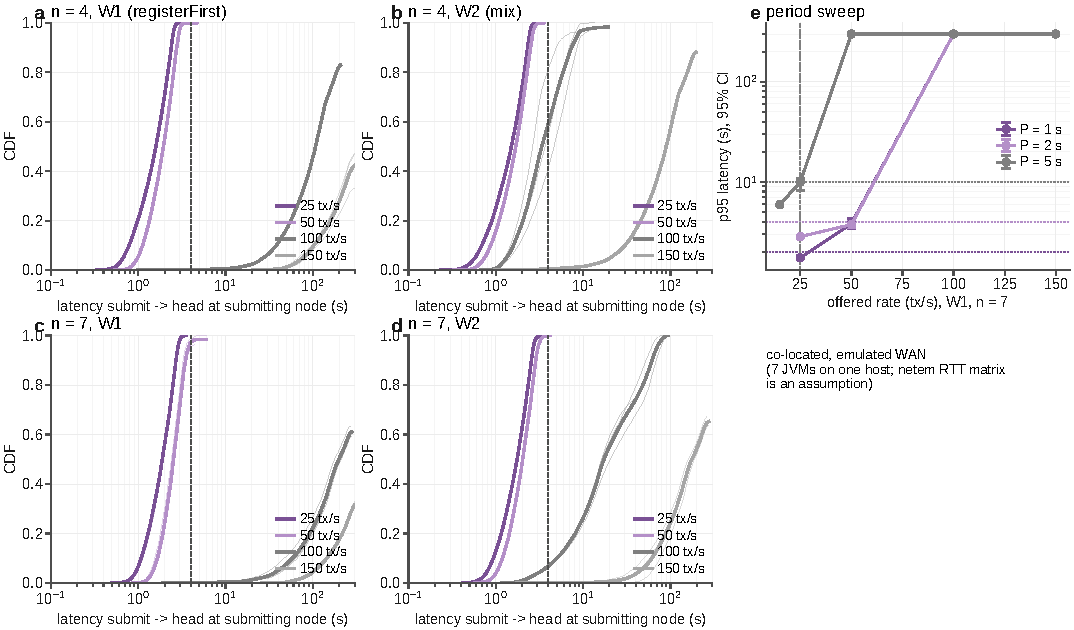
\includegraphics[width=\textwidth]{figs/fig10.pdf}
\caption{\textbf{E10 latency on the co-located Besu devnet} with emulated WAN. (a)--(d) Latency from submission to the including head
per offered rate, for $n=4$ and $n=7$ and the first-claim (W1) and mixed (W2) workloads; thin lines are single runs, the dashed line marks two
block periods. (e) 95th-percentile latency (95\% CI, capped at 300~s for display) against the offered rate for 1-, 2-
and 5-s blocks ($n=7$, W1).}
\label{fig:e10}
\end{figure}

\section{Ledger ablation (E11)}
\label{sec:e11}
Table~\ref{tab:ablation} is the summary table of the ablation (main Sec.~\mainref{sec:eval-e11}); its footer gives D's
measured inclusion latency on Besu (Table~\ref{tab:s-e11-besu}).
\begin{table}[!htbp]
\centering
\caption{\textbf{E11 ablation outcomes.} Worst outcome over the adversary sweep ($k \le f$ unless marked), $n = 4, 7$. B, C: full replayer [light client]. $\checkmark$ resisted, B bounded, R stated residual, $\odot$ detected after gossip, $\times$ succeeds; $^{\dagger}$ differs from the pre-registered prediction; $^{a}$ equals the amended prediction (grouped rows: any member). Sc5b: $k = f+1$.}
\label{tab:ablation}
\tabsmall
\setlength{\tabcolsep}{3.6pt}
\begin{tabular}{@{}lcccccclll@{}}
\toprule
Scenario & A & B(10 s) & C & C$'_{\min}$ & D & D(f+1) & Collusion (D) & Detect.\ (s) & EDR \\
\midrule
Sc1 split view & $\times$ & $\odot$ [$\times$$^{\dagger}$] & $\checkmark$ [$\times$$^{a}$] & $\checkmark$ & $\checkmark$ & $\times$ & f+1 & 5.0 / 279 & -- \\
Sc2 conflicting grants & $\times$ & $\odot$ [$\times$$^{\dagger}$] & $\checkmark$ [$\times$] & $\checkmark$ & $\checkmark$ & $\times$ & f+1 & 4.8 / 117 & 1/1 \\
Sc2 theft, Sc2b-e, Sc2d', Sc2d'' & $\times$ & $\checkmark$ [$\times$] & $\checkmark$ [$\times$] & $\checkmark$ & $\checkmark$ & $\checkmark$ & 2f+1 & -- & 10/10 \\
Sc2f, Sc2g & $\times$ & $\checkmark$ [$\times$] & $\checkmark$ [$\times$] & $\checkmark$ & $\checkmark$ & $\checkmark$ & 2f+1 & -- & 6/6 \\
Sc2f pre-proof aliases & R$^{a}$ & R$^{a}$ & R$^{a}$ & R$^{a}$ & R$^{a}$ & R$^{a}$ & 0 & -- & 1/1 \\
Sc3(i) delay d & $\times$ & $\times$ & $\times$ & B & B & $\times$ & f+1 & -- & 9/9 \\
Sc3(iii) stockpiled beacons & $\times$ & $\times$ & $\times$ & $\checkmark$ & $\checkmark$ & $\times$ & f+1 & -- & 1/1 \\
Sc3(i)/(ii)/(iv)-(vii) thief-owned & $\times$$^{\dagger}$ & $\checkmark$ [$\times$$^{\dagger}$] & $\checkmark$ [$\times$$^{\dagger}$] & $\checkmark$ & $\checkmark$ & $\checkmark$ & 2f+1 & -- & 8/8 \\
Sc3(vii) seller-owned & R & R & R & R & R & R & 0 & -- & 1/1 \\
Sc4 equivocation & $\times$ & $\odot$ [$\times$$^{\dagger}$] & $\times$$^{\dagger}$ [$\times$] & $\checkmark$ & $\checkmark$ & $\times$ & f+1 & 4.3 / 157 & 1/1 \\
Sc4' suppression & $\times$ & $\times$ & $\times$ & B & B & $\times$ & f+1 & -- & -- \\
Sc5 forged proofs & $\times$ & $\checkmark$ [$\times$] & $\checkmark$ [$\times$] & $\checkmark$ & $\checkmark$ & $\checkmark$ & 2f+1 & -- & 6/6 \\
Sc5b f+1 defamation (k = f+1 defamers) & $\times$ & $\times$ & $\times$ & $\times$ & $\times$ & $\times$ & f+1 & -- & 8/8 \\
Sc5t true failure, < f+1 checkers & $\checkmark$$^{a}$ & $\checkmark$ & $\checkmark$ & $\times$ & $\checkmark$ & $\checkmark$ & none & -- & 1/1 \\
Sc6 G, E, L, D, H, P, T & $\times$$^{a}$ & $\times$$^{\dagger}$ [$\times$$^{a}$] & $\times$$^{\dagger}$ [$\times$$^{a}$] & $\checkmark$ & $\checkmark$ & $\checkmark$ & 2f+1 & -- & 10/10 \\
\bottomrule
\end{tabular}
\tabnote{Cost per first claim on D: 228,259 gas (registerFirst \tierX{} + 1/64 anchorBatch). D latency on Besu QBFT (2-s period, n = 4, 7, k $\le$ f censoring proposers, 100 repetitions; Table~\ref{tab:s-e11-besu}): median inclusion 1.64--1.92\,s, max 5.08 s.}
\end{table}

\begin{table}[!htbp]
\centering
\caption{\textbf{Full E11 matrix.} Observed worst outcome per scenario and back end, $n=4$/$n=7$; groups $k\le f$ and $k=f+1$; B, C full replayer [light client]; D-EDR = EDR cells passing. Sc1--Sc5, Sc6 (ledger-rule cases G, E, L, D, H, P, T), Sc3-heldback and Sc2f-aliases are the pre-registered scenarios S1--S5, R4, R6D-heldback and R7E5E6-aliases of the artifact.}
\label{tab:s-e11}
\tabsmall\renewcommand{\arraystretch}{1.0}\setlength{\tabcolsep}{3.6pt}
\begin{tabular}{@{}lccccccccc@{}}
\toprule
\multicolumn{10}{l}{$k \le f$} \\
Scenario & A & B(10 s) & B(600 s) & C & C$'_{\mathrm{seq}}$ & C$'_{\min}$ & C$'_{\mathrm{native}}$ & D & D-EDR \\
\midrule
Sc1 & $\times$ & $\odot$ [$\times$$^{\dagger}$] & $\odot$ [$\times$$^{\dagger}$] & $\checkmark$ [$\times$$^{a}$] & $\checkmark$ & $\checkmark$ & $\checkmark$ & $\checkmark$ & -- \\
Sc2 & $\times$ & $\odot$ [$\times$$^{\dagger}$] & $\odot$ [$\times$$^{\dagger}$] & $\checkmark$ [$\times$] & $\checkmark$ & $\checkmark$ & $\checkmark$ & $\checkmark$ & 1/1 \\
Sc2-theft & $\times$ & $\checkmark$ [$\times$] & $\checkmark$ [$\times$] & $\checkmark$ [$\times$] & $\checkmark$ & $\checkmark$ & $\checkmark$ & $\checkmark$ & 1/1 \\
Sc2b & $\times$ & $\checkmark$ [$\times$] & $\checkmark$ [$\times$] & $\checkmark$ [$\times$] & $\checkmark$ & $\checkmark$ & $\checkmark$ & $\checkmark$ & 1/1 \\
Sc2c & $\times$ & $\checkmark$ [$\times$] & $\checkmark$ [$\times$] & $\checkmark$ [$\times$] & $\checkmark$ & $\checkmark$ & $\checkmark$ & $\checkmark$ & 2/2 \\
Sc2d & $\times$ & $\checkmark$ [$\times$] & $\checkmark$ [$\times$] & $\checkmark$ [$\times$] & $\checkmark$ & $\checkmark$ & $\checkmark$ & $\checkmark$ & 3/3 \\
Sc2d' & $\times$ & $\checkmark$ [$\times$] & $\checkmark$ [$\times$] & $\checkmark$ [$\times$] & $\checkmark$ & $\checkmark$ & $\checkmark$ & $\checkmark$ & 1/1 \\
Sc2d'' & $\times$ & $\checkmark$ [$\times$] & $\checkmark$ [$\times$] & $\checkmark$ [$\times$] & $\checkmark$ & $\checkmark$ & $\checkmark$ & $\checkmark$ & 1/1 \\
Sc2e & $\times$ & $\checkmark$ [$\times$] & $\checkmark$ [$\times$] & $\checkmark$ [$\times$] & $\checkmark$ & $\checkmark$ & $\checkmark$ & $\checkmark$ & 1/1 \\
Sc2f/P1 & $\times$ & $\checkmark$ [$\times$] & $\checkmark$ [$\times$] & $\checkmark$ [$\times$] & $\checkmark$ & $\checkmark$ & $\checkmark$ & $\checkmark$ & 2/2 \\
Sc2f/P2 & $\times$ & $\checkmark$ [$\times$] & $\checkmark$ [$\times$] & $\checkmark$ [$\times$] & $\checkmark$ & $\checkmark$ & $\checkmark$ & $\checkmark$ & 1/1 \\
Sc2f/G1 & $\times$ & $\checkmark$ [$\times$] & $\checkmark$ [$\times$] & $\checkmark$ [$\times$] & $\checkmark$ & $\checkmark$ & $\checkmark$ & $\checkmark$ & 1/1 \\
Sc2f/P3 & $\times$ & $\checkmark$ [$\times$] & $\checkmark$ [$\times$] & $\checkmark$ [$\times$] & $\checkmark$ & $\checkmark$ & $\checkmark$ & $\checkmark$ & 1/1 \\
Sc2g & $\times$ & $\checkmark$ [$\times$] & $\checkmark$ [$\times$] & $\checkmark$ [$\times$] & $\checkmark$ & $\checkmark$ & $\checkmark$ & $\checkmark$ & 1/1 \\
Sc2f-aliases & R$^{a}$ & R$^{a}$ & R$^{a}$ & R$^{a}$ & R$^{a}$ & R$^{a}$ & R$^{a}$ & R$^{a}$ & 1/1 \\
Sc3(i)/seller & $\times$ & $\times$ & $\times$ & $\times$ & $\times$ & B & B & B & 9/9 \\
Sc3(iii) & $\times$ & $\times$ & $\times$ & $\times$ & $\times$ & $\checkmark$ & $\checkmark$ & $\checkmark$ & 1/1 \\
Sc3(i)/thief & $\times$ & $\checkmark$ [$\times$] & $\checkmark$ [$\times$] & $\checkmark$ [$\times$] & $\checkmark$ & $\checkmark$ & $\checkmark$ & $\checkmark$ & -- \\
Sc3(ii) & $\times$ & $\checkmark$ [$\times$] & $\checkmark$ [$\times$] & $\checkmark$ [$\times$] & $\checkmark$ & $\checkmark$ & $\checkmark$ & $\checkmark$ & 1/1 \\
Sc3(iv) & $\times$ & $\checkmark$ [$\times$] & $\checkmark$ [$\times$] & $\checkmark$ [$\times$] & $\checkmark$ & $\checkmark$ & $\checkmark$ & $\checkmark$ & 1/1 \\
Sc3(v) & $\times$ & $\checkmark$ [$\times$] & $\checkmark$ [$\times$] & $\checkmark$ [$\times$] & $\checkmark$ & $\checkmark$ & $\checkmark$ & $\checkmark$ & 1/1 \\
Sc3(vi) & $\times$ & $\checkmark$ [$\times$] & $\checkmark$ [$\times$] & $\checkmark$ [$\times$] & $\checkmark$ & $\checkmark$ & $\checkmark$ & $\checkmark$ & 1/1 \\
Sc3(vii)/thief & $\times$ & $\checkmark$ [$\times$] & $\checkmark$ [$\times$] & $\checkmark$ [$\times$] & $\checkmark$ & $\checkmark$ & $\checkmark$ & $\checkmark$ & 3/3 \\
Sc3-heldback & $\checkmark$$^{\dagger}$ & $\checkmark$ [$\checkmark$$^{\dagger}$] & $\checkmark$ [$\checkmark$$^{\dagger}$] & $\checkmark$ [$\checkmark$$^{\dagger}$] & $\checkmark$ & $\checkmark$ & $\checkmark$ & $\checkmark$ & 1/1 \\
Sc3(vii)/seller & R & R & R & R & R & R & R & R & 1/1 \\
Sc4 & $\times$ & $\odot$ [$\times$$^{\dagger}$] & $\odot$ [$\times$$^{\dagger}$] & $\times$$^{\dagger}$ [$\times$] & $\times$$^{\dagger}$ & $\checkmark$ & $\checkmark$ & $\checkmark$ & 1/1 \\
Sc4' & $\times$ & $\times$ & $\times$ & $\times$ & $\times$ & B & B & B & -- \\
Sc5 & $\times$ & $\checkmark$ [$\times$] & $\checkmark$ [$\times$] & $\checkmark$ [$\times$] & $\checkmark$ & $\checkmark$ & $\checkmark$ & $\checkmark$ & 6/6 \\
Sc5b/n4 & $\checkmark$$^{a}$ & $\checkmark$$^{a}$ & $\checkmark$$^{a}$ & $\checkmark$$^{a}$ & $\checkmark$$^{a}$ & $\checkmark$$^{a}$ & $\checkmark$$^{a}$ & $\checkmark$$^{a}$ & 1/1 \\
Sc5b/n7 & $\checkmark$$^{a}$ & $\checkmark$$^{a}$ & $\checkmark$$^{a}$ & $\checkmark$$^{a}$ & $\checkmark$$^{a}$ & $\checkmark$ & $\checkmark$ & $\checkmark$ & 7/7 \\
Sc5t & $\checkmark$$^{a}$ & $\checkmark$ [$\checkmark$$^{a}$] & $\checkmark$ [$\checkmark$$^{a}$] & $\checkmark$ [$\checkmark$$^{a}$] & $\times$ & $\times$ & $\checkmark$ & $\checkmark$ & 1/1 \\
Sc6/G & $\times$ & $\checkmark$ [$\times$] & $\checkmark$ [$\times$] & $\checkmark$ [$\times$] & $\checkmark$ & $\checkmark$ & $\checkmark$ & $\checkmark$ & 3/3 \\
Sc6/E & $\times$ & $\times$$^{\dagger}$ [$\times$] & $\times$$^{\dagger}$ [$\times$] & $\times$$^{\dagger}$ [$\times$] & $\times$$^{\dagger}$ & $\checkmark$ & $\checkmark$ & $\checkmark$ & 1/1 \\
Sc6/L & $\times$ & $\checkmark$ [$\times$] & $\checkmark$ [$\times$] & $\checkmark$ [$\times$] & $\checkmark$ & $\checkmark$ & $\checkmark$ & $\checkmark$ & 1/1 \\
Sc6/D & $\times$ & $\checkmark$ [$\times$] & $\checkmark$ [$\times$] & $\checkmark$ [$\times$] & $\checkmark$ & $\checkmark$ & $\checkmark$ & $\checkmark$ & 2/2 \\
Sc6/H & $\checkmark$$^{a}$ & $\checkmark$ [$\checkmark$$^{a}$] & $\checkmark$ [$\checkmark$$^{a}$] & $\checkmark$ [$\checkmark$$^{a}$] & $\checkmark$ & $\checkmark$ & $\checkmark$ & $\checkmark$ & 1/1 \\
Sc6/P & $\times$ & $\checkmark$ [$\times$] & $\checkmark$ [$\times$] & $\checkmark$ [$\times$] & $\checkmark$ & $\checkmark$ & $\checkmark$ & $\checkmark$ & 1/1 \\
Sc6/T & $\times$ & $\checkmark$ [$\times$] & $\checkmark$ [$\times$] & $\checkmark$ [$\times$] & $\checkmark$ & $\checkmark$ & $\checkmark$ & $\checkmark$ & 1/1 \\
\midrule
\end{tabular}
\\[4pt]
\begin{tabular}{@{}lccccccccc@{}}
\midrule
\multicolumn{10}{l}{$k = f+1$} \\
Scenario & A & B(10 s) & B(600 s) & C & C$'_{\mathrm{seq}}$ & C$'_{\min}$ & C$'_{\mathrm{native}}$ & D & D-EDR \\
\midrule
Sc1 & -- & -- & -- & $\odot$ [$\times$$^{a}$] & $\times$ & $\times$ & $\times$ & $\times$ & -- \\
Sc2 & -- & -- & -- & $\odot$ [$\times$] & $\times$ & $\times$ & $\times$ & $\times$ & 1/1 \\
Sc2-theft & -- & -- & -- & $\checkmark$ [$\times$] & $\checkmark$ & $\checkmark$ & $\checkmark$ & $\checkmark$ & 1/1 \\
Sc2b & -- & -- & -- & $\checkmark$ [$\times$] & $\checkmark$ & $\checkmark$ & $\checkmark$ & $\checkmark$ & 1/1 \\
Sc2c & -- & -- & -- & $\checkmark$ [$\times$] & $\checkmark$ & $\checkmark$ & $\checkmark$ & $\checkmark$ & 2/2 \\
Sc2d & -- & -- & -- & $\checkmark$ [$\times$] & $\checkmark$ & $\checkmark$ & $\checkmark$ & $\checkmark$ & 3/3 \\
Sc2d' & -- & -- & -- & $\checkmark$ [$\times$] & $\checkmark$ & $\checkmark$ & $\checkmark$ & $\checkmark$ & 1/1 \\
Sc2d'' & -- & -- & -- & $\checkmark$ [$\times$] & $\checkmark$ & $\checkmark$ & $\checkmark$ & $\checkmark$ & 1/1 \\
Sc2e & -- & -- & -- & $\checkmark$ [$\times$] & $\checkmark$ & $\checkmark$ & $\checkmark$ & $\checkmark$ & 1/1 \\
Sc2f/P1 & -- & -- & -- & $\checkmark$ [$\times$] & $\checkmark$ & $\checkmark$ & $\checkmark$ & $\checkmark$ & 2/2 \\
Sc2f/P2 & -- & -- & -- & $\checkmark$ [$\times$] & $\checkmark$ & $\checkmark$ & $\checkmark$ & $\checkmark$ & 1/1 \\
Sc2f/G1 & -- & -- & -- & $\checkmark$ [$\times$] & $\checkmark$ & $\checkmark$ & $\checkmark$ & $\checkmark$ & 1/1 \\
Sc2f/P3 & -- & -- & -- & $\checkmark$ [$\times$] & $\checkmark$ & $\checkmark$ & $\checkmark$ & $\checkmark$ & 1/1 \\
Sc2g & -- & -- & -- & $\checkmark$ [$\times$] & $\checkmark$ & $\checkmark$ & $\checkmark$ & $\checkmark$ & 1/1 \\
Sc2f-aliases & -- & -- & -- & R$^{a}$ & R$^{a}$ & R$^{a}$ & R$^{a}$ & R$^{a}$ & 1/1 \\
Sc3(i)/seller & -- & -- & -- & $\times$ & $\times$ & $\times$ & $\times$ & $\times$ & 9/9 \\
Sc3(iii) & -- & -- & -- & $\times$ & $\times$ & $\times$ & $\times$ & $\times$ & 1/1 \\
Sc3(i)/thief & -- & -- & -- & $\checkmark$ [$\times$] & $\checkmark$ & $\checkmark$ & $\checkmark$ & $\checkmark$ & -- \\
Sc3(ii) & -- & -- & -- & $\checkmark$ [$\times$] & $\checkmark$ & $\checkmark$ & $\checkmark$ & $\checkmark$ & 1/1 \\
Sc3(iv) & -- & -- & -- & $\checkmark$ [$\times$] & $\checkmark$ & $\checkmark$ & $\checkmark$ & $\checkmark$ & 1/1 \\
Sc3(v) & -- & -- & -- & $\checkmark$ [$\times$] & $\checkmark$ & $\checkmark$ & $\checkmark$ & $\checkmark$ & 1/1 \\
Sc3(vi) & -- & -- & -- & $\checkmark$ [$\times$] & $\checkmark$ & $\checkmark$ & $\checkmark$ & $\checkmark$ & 1/1 \\
Sc3(vii)/thief & -- & -- & -- & $\checkmark$ [$\times$] & $\checkmark$ & $\checkmark$ & $\checkmark$ & $\checkmark$ & 3/3 \\
Sc3-heldback & -- & -- & -- & $\checkmark$ [$\checkmark$$^{\dagger}$] & $\checkmark$ & $\checkmark$ & $\checkmark$ & $\checkmark$ & 1/1 \\
Sc3(vii)/seller & -- & -- & -- & R & R & R & R & R & 1/1 \\
Sc4 & -- & -- & -- & $\odot$ [$\times$] & $\times$ & $\times$ & $\times$ & $\times$ & 1/1 \\
Sc4' & -- & -- & -- & $\times$ & $\times$ & $\times$ & $\times$ & $\times$ & -- \\
Sc5 & -- & -- & -- & $\checkmark$ [$\times$] & $\checkmark$ & $\checkmark$ & $\checkmark$ & $\checkmark$ & 6/6 \\
Sc5b/n4 & $\times$ & $\times$ & $\times$ & $\times$ & $\times$ & $\times$ & $\times$ & $\times$ & 1/1 \\
Sc5b/n7 & $\times$ & $\times$ & $\times$ & $\times$ & $\times$ & $\times$ & $\times$ & $\times$ & 7/7 \\
Sc5t & -- & -- & -- & $\checkmark$ [$\checkmark$$^{a}$] & $\times$ & $\times$ & $\checkmark$ & $\checkmark$ & 1/1 \\
Sc6/G & -- & -- & -- & $\checkmark$ [$\times$] & $\checkmark$ & $\checkmark$ & $\checkmark$ & $\checkmark$ & 3/3 \\
Sc6/E & -- & -- & -- & $\times$$^{\dagger}$ [$\times$] & $\times$$^{\dagger}$ & $\checkmark$ & $\checkmark$ & $\checkmark$ & 1/1 \\
Sc6/L & -- & -- & -- & $\checkmark$ [$\times$] & $\checkmark$ & $\checkmark$ & $\checkmark$ & $\checkmark$ & 1/1 \\
Sc6/D & -- & -- & -- & $\checkmark$ [$\times$] & $\checkmark$ & $\checkmark$ & $\checkmark$ & $\checkmark$ & 2/2 \\
Sc6/H & -- & -- & -- & $\checkmark$ [$\checkmark$$^{a}$] & $\checkmark$ & $\checkmark$ & $\checkmark$ & $\checkmark$ & 1/1 \\
Sc6/P & -- & -- & -- & $\checkmark$ [$\times$] & $\checkmark$ & $\checkmark$ & $\checkmark$ & $\checkmark$ & 1/1 \\
Sc6/T & -- & -- & -- & $\checkmark$ [$\times$] & $\checkmark$ & $\checkmark$ & $\checkmark$ & $\checkmark$ & 1/1 \\
\bottomrule
\end{tabular}
\end{table}

\begin{table}[!htbp]
\centering
\caption{\textbf{E11 back end D on Besu QBFT.} Inclusion delay with $k$ censoring proposers (20 repetitions) vs.\ the D-model bound $(k+1)\cdot 2$\,s.}
\label{tab:s-e11-besu}
\tabsize
\begin{tabular}{@{}rrrrrrrr@{}}
\toprule
$n$ & $k$ & Reps & Median (s) & p95 (s) & Max (s) & Bound (s) & $>$Bound \\
\midrule
4 & 0 & 20 & 1.64 & 2.35 & 2.35 & 2 & 6 \\
4 & 1 & 20 & 1.87 & 4.22 & 4.22 & 4 & 1 \\
7 & 0 & 20 & 1.71 & 2.59 & 2.59 & 2 & 6 \\
7 & 1 & 20 & 1.86 & 4.01 & 4.01 & 4 & 1 \\
7 & 2 & 20 & 1.92 & 5.08 & 5.08 & 6 & 0 \\
\bottomrule
\end{tabular}
\end{table}

\begin{figure}[!htbp]
\centering
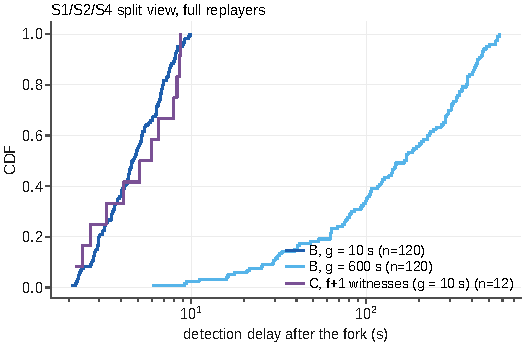
\includegraphics[width=0.5\textwidth]{figs/fig_s_e11_detect.pdf}
\caption{\textbf{E11: equivocation detection.} Back end B's detection time against the gossip period.}
\label{fig:s-e11-detect}
\end{figure}

\begin{figure}[!htbp]
\centering
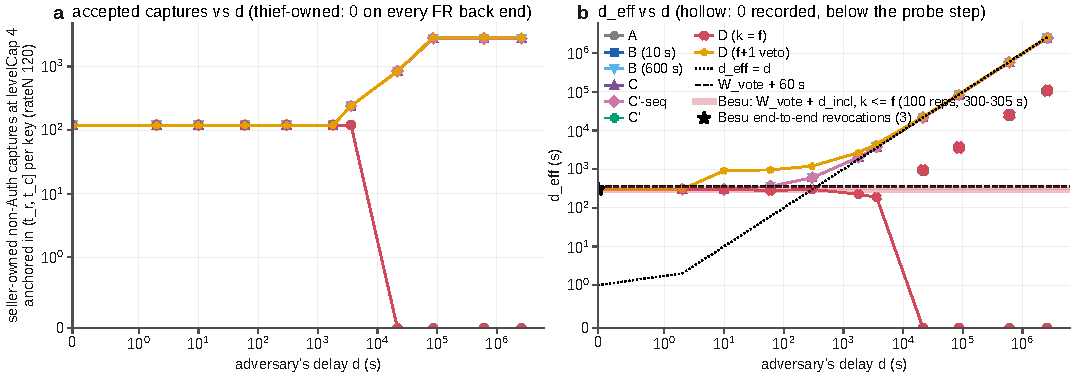
\includegraphics[width=\textwidth]{figs/fig_s_e11_s3curve.pdf}
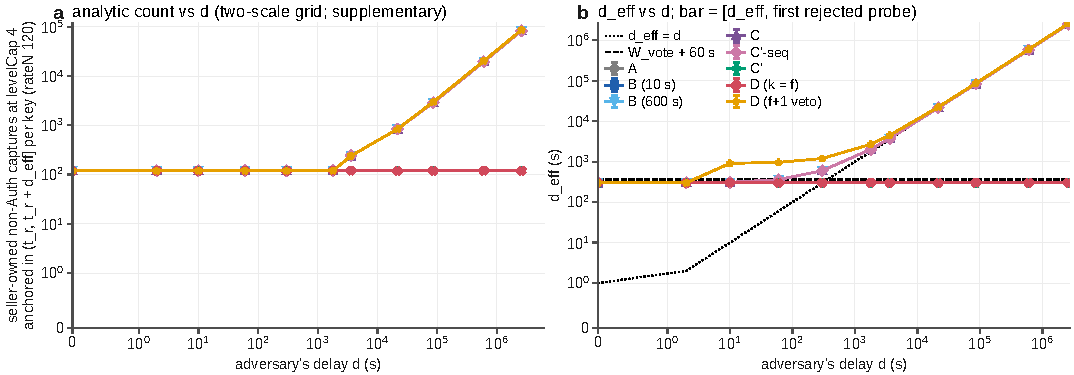
\includegraphics[width=\textwidth]{figs/fig_s_e11_s3curve_2scale.pdf}
\caption{\textbf{E11 Sc3 backdating window} against the operator delay. Top: pre-registered probe grid (with its resolution
limit). Bottom: the two-scale grid applied after the freeze (disclosed), which gives C$'$ and D a window of 303--310~s
at every delay.}
\label{fig:s-e11-s3}
\end{figure}
\textbf{Model bound.} On Besu, 14 of 100 censored repetitions exceeded the D-model's registered inclusion bound
$(k+1)\cdot2$~s by at most 0.586~s (6 of 20 at $k=0$ for each $n$, 1 of 20 at $k=1$, none at $n=7$, $k=2$); all are
within $(k+2)\cdot2$~s. Exit row 11 stays FAIL as written; the $(k+2)$-period envelope is recorded as a disclosed
revision of the model bound for the paper's model description, and the frozen bound, comparison and scores are
unchanged.

\section{Costs, storage and timing (E12, E16, E16b)}
\label{sec:e12}
\begin{table}[!htbp]
\centering
\caption{\textbf{E12 costs and storage.} Quiet re-run (disclosed deviation: run 1 ran on a loaded shared host, every line load-flagged; both are reported). Medians over masters of per-master medians of 1-thread runs; times in ms unless marked. Fast = numpy Compile plus libjpeg-turbo re-encode (no native verifier was built); its design target $\le$ 20 ms/MP is a reported comparison. Capture at 4-12 MP is inflated by OpenCV threading under the one-core quota (E16b: 2.95 s at 12 MP with one thread). $^{u}$Upscaled masters are Lanczos-upscaled natives. Evaluate excludes PubSeg inference (priced by E5). Load-average flags ($>$ 2.0): 8.}
\label{tab:costs}
\tabsmall
\setlength{\tabcolsep}{2.6pt}
\begin{tabular}{@{}lrrrrrrrrrrrrrrr@{}}
\toprule
& & & Capture & Compile & \Ezero{} enc. & \VerifyE{} & Fast & Fast & \Evaluate{} & Hop & Opened & Bundle & $U$ rec & Store/cap & Store/list \\
Master & Listing (px) & $n$ & (s) & (ms) & (ms) & py (ms) & (ms) & (ms/MP) & (ms) & (ms) & (KiB) & (KiB) & (KiB) & (MiB) & (KiB) \\
\midrule
0.5 MP & 512 & 8 & 0.08 & 48.2 & 4.5 & 140.3 & 63.1 & 289.5 & 157.8 & 60.0 & 374.0 & 414.4 & 49.0 & 1.41 & 497.2 \\
0.5 MP & 1024 & 2 & 0.08 & 95.3 & 9.6 & 282.8 & 124.8 & 274.3 & 320.7 & 105.1 & 562.8 & 654.3 & 111.5 & 1.41 & 855.0 \\
1 MP & 512 & 9 & 0.17 & 31.3 & 4.1 & 100.5 & 39.6 & 294.3 & 111.8 & 35.4 & 246.3 & 285.2 & 32.0 & 2.82 & 360.2 \\
1 MP & 1024 & 5 & 0.17 & 126.7 & 10.1 & 358.8 & 162.5 & 307.1 & 398.2 & 108.4 & 792.8 & 903.1 & 119.7 & 2.82 & 1155.6 \\
2 MP & 512 & 9 & 0.60 & 45.5 & 4.4 & 132.9 & 57.5 & 277.2 & 147.9 & 56.9 & 268.0 & 299.7 & 46.8 & 4.34 & 373.8 \\
2 MP & 1024 & 9 & 0.60 & 181.9 & 13.3 & 480.4 & 219.5 & 289.9 & 539.3 & 153.6 & 887.0 & 980.3 & 170.7 & 4.34 & 1240.4 \\
4 MP & 512 & 10 & 1.61 & 41.0 & 4.2 & 129.5 & 52.0 & 283.9 & 143.4 & 60.0 & 269.4 & 302.4 & 47.9 & 7.62 & 390.4 \\
4 MP & 1024 & 9 & 1.61 & 148.3 & 13.1 & 458.8 & 187.9 & 307.2 & 512.2 & 147.8 & 1288.7 & 1367.1 & 181.6 & 7.62 & 1637.1 \\
4 MP & 2048 & 4 & 1.61 & 573.4 & 43.7 & 1578.2 & 699.4 & 235.7 & 1805.7 & 308.4 & 1532.1 & 1785.5 & 698.8 & 7.62 & 2585.5 \\
8 MP$^{u}$ & 512 & 9 & 4.83 & 43.7 & 5.3 & 129.6 & 56.1 & 268.3 & 145.1 & 55.2 & 229.8 & 268.5 & 49.0 & 23.16 & 353.8 \\
8 MP$^{u}$ & 1024 & 9 & 4.83 & 147.4 & 13.3 & 430.3 & 189.0 & 260.1 & 484.5 & 146.7 & 789.2 & 889.0 & 177.5 & 23.16 & 1163.8 \\
8 MP$^{u}$ & 2048 & 10 & 4.83 & 585.2 & 51.5 & 1679.2 & 742.4 & 257.0 & 1936.7 & 310.9 & 2941.5 & 3253.8 & 702.9 & 23.16 & 4335.6 \\
12 MP$^{u}$ & 512 & 7 & 9.80 & 34.4 & 4.0 & 109.8 & 46.5 & 292.1 & 125.3 & 55.7 & 273.1 & 307.8 & 49.0 & 25.54 & 378.5 \\
12 MP$^{u}$ & 1024 & 8 & 9.80 & 148.2 & 12.5 & 440.6 & 189.1 & 291.0 & 495.7 & 147.6 & 1060.4 & 1148.4 & 176.8 & 25.54 & 1366.2 \\
12 MP$^{u}$ & 2048 & 9 & 9.80 & 617.4 & 41.8 & 1861.7 & 768.9 & 286.8 & 2109.7 & 294.9 & 3908.0 & 4149.5 & 658.2 & 25.54 & 4860.0 \\
\bottomrule
\end{tabular}
\end{table}

\begin{table}[!htbp]
\centering\tabsize
\caption{\textbf{E12 quiet run and loaded run.} Quiet run (primary) and run~1 (loaded host, disclosed) for selected cells: medians in ms unless marked.}
\label{tab:e12-runs}
\setlength{\tabcolsep}{4pt}
\begin{tabular}{@{}llcrrrrrrr@{}}
\toprule
Master & Listing (px) & Run & Capture (s) & Compile & \VerifyE{} py & Fast & Fast (ms/MP) & \Evaluate{} & Hop \\
\midrule
0.5 MP & 512 & quiet & 0.08 & 48.2 & 140.3 & 63.1 & 289.5 & 157.8 & 60.0 \\
0.5 MP & 512 & run 1 & 0.09 & 50.7 & 144.0 & 63.2 & 297.5 & 162.6 & 52.8 \\
\addlinespace[2pt]
1 MP & 1024 & quiet & 0.17 & 126.7 & 358.8 & 162.5 & 307.1 & 398.2 & 108.4 \\
1 MP & 1024 & run 1 & 0.18 & 137.3 & 385.7 & 176.7 & 327.7 & 438.5 & 117.8 \\
\addlinespace[2pt]
4 MP & 1024 & quiet & 1.61 & 148.3 & 458.8 & 187.9 & 307.2 & 512.2 & 147.8 \\
4 MP & 1024 & run 1 & 1.12 & 164.0 & 520.0 & 205.7 & 324.4 & 584.2 & 164.4 \\
\addlinespace[2pt]
4 MP & 2048 & quiet & 1.61 & 573.4 & 1578.2 & 699.4 & 235.7 & 1805.7 & 308.4 \\
4 MP & 2048 & run 1 & 1.12 & 661.6 & 1735.2 & 772.2 & 260.7 & 1964.2 & 366.3 \\
\addlinespace[2pt]
12 MP & 1024 & quiet & 9.80 & 148.2 & 440.6 & 189.1 & 291.0 & 495.7 & 147.6 \\
12 MP & 1024 & run 1 & 5.40 & 211.6 & 618.8 & 268.1 & 327.8 & 696.0 & 190.4 \\
\addlinespace[2pt]
12 MP & 2048 & quiet & 9.80 & 617.4 & 1861.7 & 768.9 & 286.8 & 2109.7 & 294.9 \\
12 MP & 2048 & run 1 & 5.40 & 734.4 & 2129.3 & 916.6 & 354.4 & 2484.7 & 326.6 \\
\bottomrule
\end{tabular}
\end{table}
Run~1 ran on a loaded shared host (all 60 lines flagged, median 1-min load maximum 6.42); the quiet rerun has 8 of 60
lines flagged (median 1.45), which were not repeated. Storage bytes are identical in both runs. The capture commit at
4 and 12~MP was slower in the quiet run; E16b (below) confirms the cause: OpenCV's thread pool under the one-core quota.

\textbf{Profile (E16).} One master per size, single thread, run while other jobs loaded the host (1-min load 3--7):
ratios are reliable, absolute times indicative only. The ``fast path'' is the numpy \Compile{} plus the libjpeg-turbo
re-encode and compare; no native (C) verifier was built.
\begin{table}[!htbp]
\centering\tabsize
\caption{\textbf{E16 fast-path profile} (one master per size, loaded host).}
\label{tab:x4}
\begin{tabular}{@{}llrrrrr@{}}
\toprule
Master & Listing (px) & Canvas (MP) & Fast path (ms) & \Compile{} (ms) & libjpeg encode (ms) & Encode (ms/MP) \\
\midrule
4 MP & 1024 & 0.74 & 250.5 & 207.6 & 14.0 & 18.8 \\
4 MP & 2048 & 2.90 & 920.7 & 810.6 & 51.3 & 17.7 \\
12 MP & 1024 & 0.63 & 176.3 & 129.7 & 12.9 & 20.6 \\
12 MP & 2048 & 2.43 & 1113.8 & 954.1 & 44.6 & 18.4 \\
12 MP & 512 & 0.17 & 54.6 & 39.0 & 4.3 & 26.2 \\
\bottomrule
\end{tabular}
\end{table}
The numpy \Compile{} takes 74--88\% of the fast path at 1024- and 2048-px listings, and the libjpeg-turbo encode
17.7--20.6~ms/MP there (22--31 at 512~px). Prediction (1) holds in part: \Compile{} dominates, but the encode is about
20~ms/MP, not well below. A native verifier was not built; the encode alone indicates the order of magnitude of a native
verifier's encoding step, not its total cost. Per $10^6$ 1024-px listings: fast path about 49--70 CPU-hours, the integer Python \VerifyE{} 113--151, the encode
alone 3.6--3.9. Prediction (2) fails: the 12-MP capture commit (6.0--6.6~s) is dominated by OpenCV's elliptical dilation of the
certified region (3.8~s, of which \texttt{cv2.dilate} 3.58~s), with cell hashing 2.8~s, and a first-call gap appears
only at 0.5~MP. OpenCV's thread pool is not pinned by \texttt{OMP\_NUM\_THREADS}.

\textbf{E16b: quiet host and thread test.} Registered after E16's result and committed before its run, E16b re-ran E16
alone on a quiet host (5-min load below 1.0 at the start; no line above a 1-min load of 2.0)
under the same one-core CPU quota as E12 and E16, and timed the 12-MP capture commit and the dilation alone six times
each with OpenCV's default 12 threads and with one thread (ABBA order). Quiet fast path at listings $\ge1024$~px:
223--366~ms/MP (E16 under load: 282--458); libjpeg encode 17.1--19.3~ms/MP, 5--9\% of the fast path. Capture commit at
12~MP: 9.78~s with default threads (E12 quiet: 9.80~s); default vs one thread 9.99 vs 2.95~s ($3.4\times$), dilation
7.66 vs 0.80~s ($9.6\times$), with a median 84.8~s of throttled CPU time per capture against $\approx0$. The registered
criterion (ratios $\ge1.25$ with more throttling) confirms the threading explanation: under a one-core quota the
12-thread pool is throttled and burns CPU in parallel overhead, and on a loaded host fewer of its threads run at once.
Without a quota, 12 threads take 2.38~s and one thread 2.94~s. The single-thread 2.95~s is the comparable one-core cost
of a 12-MP capture commit; the 4--12-MP capture commits of E12 and E16 are artefacts of this interaction.

\section{Worked example of a certified listing}
\label{sec:example}
Fig.~\ref{fig:example} shows, on a schematic \G{3} listing, which MCUs are certified, which are declared and where the drawn silhouette is eroded.
\begin{figure}[!htbp]
\centering
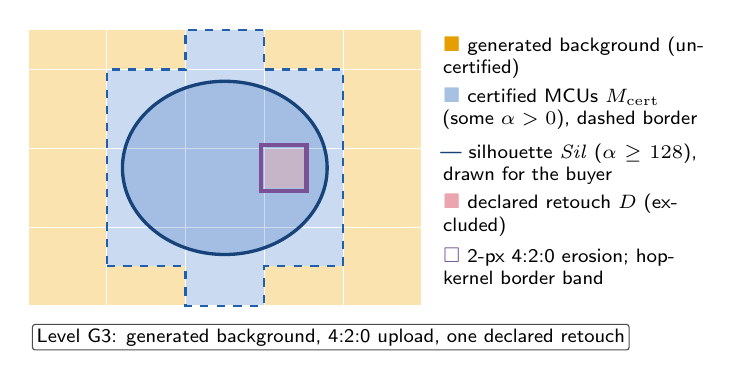
\begin{tikzpicture}[x=0.5cm,y=0.5cm,font=\sffamily\scriptsize]
\fill[cutgenlight] (0,0) rectangle (10,7);
\foreach \i/\j in {2/1,2/2,2/3,2/4,2/5,3/1,3/2,3/3,3/4,3/5,4/0,4/1,4/2,4/3,4/4,4/5,4/6,5/0,5/1,5/2,5/3,5/4,5/5,5/6,6/1,6/2,6/3,6/4,6/5,7/1,7/2,7/3,7/4,7/5}
  \fill[cutaccentlight] (\i,\j) rectangle ++(1,1);
\fill[white] (6,3) rectangle (7,4);
\fill[cutfaillight] (6,3) rectangle (7,4);
\draw[white,very thin] (0,0) grid (10,7);
\fill[cutaccent,opacity=0.22] (5,3.5) ellipse (2.6 and 2.2);
\draw[very thick,cutaccent!70!black] (5,3.5) ellipse (2.6 and 2.2);
\draw[cutledger,line width=1.6pt] (5.92,2.92) rectangle (7.08,4.08);
\draw[dashed,thick,cutaccent] (2,1) -- (4,1) -- (4,0) -- (6,0) -- (6,1) -- (8,1) -- (8,6) -- (6,6) -- (6,7) -- (4,7) -- (4,6) -- (2,6) -- cycle;
\node[anchor=west,align=left,text width=3.3cm] at (10.3,6.3) {\textcolor{cutgen}{$\blacksquare$} generated background (uncertified)};
\node[anchor=west,align=left,text width=3.3cm] at (10.3,5.0) {\textcolor{cutaccentlight!80!cutaccent}{$\blacksquare$} certified MCUs $\Mcert$ (some $\alpha>0$), dashed border};
\node[anchor=west,align=left,text width=3.3cm] at (10.3,3.6) {\textcolor{cutaccent!70!black}{\textbf{---}} silhouette $\Sil$ ($\alpha\ge128$), drawn for the buyer};
\node[anchor=west,align=left,text width=3.3cm] at (10.3,2.3) {\textcolor{cutfaillight!70!cutfail}{$\blacksquare$} declared retouch $D$ (excluded)};
\node[anchor=west,align=left,text width=3.3cm] at (10.3,1.0) {\textcolor{cutledger}{$\square$} 2-px 4:2:0 erosion; hop-kernel border band};
\node[anchor=west,draw=cutgrey,rounded corners=1pt,fill=white,inner sep=1.5pt] at (0.1,-0.8) {Level \G{3}: generated background, 4:2:0 upload, one declared retouch};
\end{tikzpicture}
\caption{\textbf{Worked example of a \G{3} listing} (schematic; one square is one $16\times16$ MCU; main Fig.~2 shows a real example). The generated background and $D$ are not certified. The drawn silhouette
excludes $D$ and, at 4:2:0, is eroded by 2~px along borders between certified and uncertified MCUs (violet frame; here only
the border with $D$, since $\Sil$ stays inside the outer certified border); after a resampling
hop, pixels whose kernel footprint leaves $\Mcert$ are not bounded (main Proposition~\mainref{prop:hops}).}
\label{fig:example}
\end{figure}

\section{System architecture}
\label{sec:arch}
Fig.~\ref{fig:system} shows \sys{} end to end; the numbered arrows follow the workflow of main Sec.~\mainref{sec:overview}
(1--2 capture, 3--5 compile and upload, 6--7 hops, 8 adjudication, 9 evaluation).
\begin{figure*}[!t]
\centering
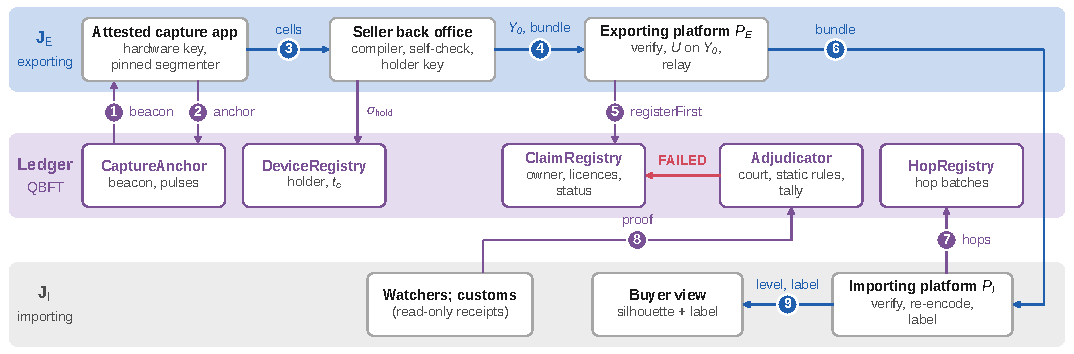
\includegraphics[width=\textwidth]{figs/fig6_arch_detail.pdf}
\caption{\textbf{\sys{} architecture.} Top: the exporting jurisdiction $J_E$; middle: the consortium ledger (one validator per
regulatory bloc); bottom: importing jurisdictions $J_I$. Only roots and status go on chain; the claim bundle (product
cells at most $2\times$ listing resolution and the public background) goes to $P_I$; masters, unopened cells, salts and
identities never leave $J_E$.}
\label{fig:system}
\end{figure*}

\section{Ledger details}
\label{sec:ledger-details}
This section expands main Sec.~\mainref{sec:ledger}.
\textbf{Consortium parameters.} Besu QBFT with $n=7$ validators in seven regulatory blocs, at most one seat per bloc
(the EU counts as one), 2-s blocks and a block gas limit of 30~M gas; at $n=4$ any two colluding blocs can break safety or censor.
We use an EVM chain for off-the-shelf tooling, the P-256 verification precompile and a programmable court. The nine
registry contracts are each below 24,576 bytes.

\textbf{Court, path (a): single-MCU proof.} For a 4:4:4 \tierXa{} claim the proof carries one failing MCU with its
coefficients and $\RY$ path, the covering cells (at most $3\times3$ by static rule~3) with their paths, the background
leaf if the block's minimum alpha is below 255, and the program. The court lets receipt-only parties (customs, small
platforms) see FAILED and makes one honest watcher's verdict binding everywhere, in the any-trust sense of
Arbitrum~\cite{kalodner2018arbitrum}. Equivalence of the contract with the reference predicate (\AS{10}) was tested on
22,306 cases (main Sec.~\mainref{sec:eval-e9}). A proof costs about $21{,}000+40$ gas per non-zero calldata byte under
the EIP-7623 floor~\cite{eip2024eip7623}, at most 1.0~M gas for captures up to 12~MP with at most 45 declared retouched
MCUs, and 14,349,680 gas at the adversarial size bound of static rule~9, below the 16,777,216-gas per-transaction
cap~\cite{eip2024eip7825}, so gas never blocks a proof. Transaction size can: that bound case (measured on EDR only) carries
416,324 calldata bytes, so validators must admit transactions above Besu's default pool limit of 131,072~bytes. With
the limit raised to 1,048,576~bytes, the 289,028-byte proof of the 12-MP case with 65,535 declared MCUs (E17b) was
mined on Besu (\S\ref{sec:e9-gas}). Violations of static rules 1--9 are proven in
$O(1)$: the proof names the rule and the offending entry and costs 105,186--128,185 gas including the strike.

\textbf{Court, path (b): tallied verdicts.} Validators run the pinned checker on claims the court cannot check (4:2:0,
fallback tier) and vote transcripts within $\Wvote=150$ blocks under the tally rule of main
Sec.~\mainref{sec:ledger}; a defamation by $f+1$ colluders is cleared by appeal at $n\ge7$. Uploads at 4:2:0 are capped
at \G{3}.

\textbf{Alternative: signed captures and transcode manifests.} Camera signing~\cite{gosb2025pixel} plus platform-signed
C2PA transcode actions (\texttt{c2pa.transcoded}~\cite{cfcpaa2026content}) need no openings or ledger but trust every transcoder,
leave region and composite self-declared, and keep status per validator~\cite{golaszewski2026verifying}.

\textbf{Status and receipts.} The ledger cap is 0 for an unknown claim or a key invalid at the anchor, 1 if the claim's
principal is struck, the claim is withdrawn or its claimant is no longer authorised, 2 if the capture is
time-unverified, and 4 otherwise. Parties without a node use receipts (a header with $2f+1$ commit seals plus storage
proofs), accepted only within 30 blocks of a head reported by $f+1$ validators and within 5~min of wall-clock time;
a stale receipt yields ``status unknown'' (\G{2}). A receipt-only party that does not run \VerifyE{} never shows a
\G{3}/\G{4} label.

\textbf{Labels.} Labels are per-jurisdiction tables, monotone in the level, that pin \G{0}/\G{1} to the regime's ``no
provenance information'' code.

\textbf{Privacy.} On chain there are only salted or keyed digests, per-capture owner pseudonyms and status; since salted
hashes count as personal data~\cite{edpb2026blockchain}, erasure deletes the off-chain salts and bundles. Masters,
unopened cells and identities never leave $J_E$; all captures of one device remain linkable.

\textbf{Costs.} The canonical first-claim cost (capture registration plus claim, evaluated build) is 226,682 gas on Besu,
about 132 per block of 30~M gas by gas arithmetic. Variants of the same operation: 226,668--226,692 on EDR (calldata bytes
and the signature's $v$ value differ); 234,288 on average under the E10 load (Table~\ref{tab:gas}); and 228,259 in the
ablation summary, which adds a $1/64$ share of an anchor batch (Table~\ref{tab:ablation}).

\section{Positioning: full table}
\label{sec:positioning-full}
Table~\ref{tab:positioning} places \sys{} against the closest lines of work.
\begin{landscape}
{\tabsmall\setlength{\tabcolsep}{3.5pt}\sloppy
\begin{longtable}{@{}L{2.9cm}L{2.2cm}L{2.5cm}L{1.9cm}L{3.2cm}L{1.9cm}L{5.0cm}L{2.2cm}@{}}
\caption{\textbf{Positioning and breaks by design.} Published costs are quoted with their page or table.}\label{tab:positioning}\\
\toprule
Line of work & Reference needed at verification & Lossy codec & Partial disclosure & Adversarial guarantee & Re-encode tolerance & Cost (as published) & E4 (this paper) \\
\midrule
\endfirsthead
\multicolumn{8}{@{}l}{\small\itshape Table~\thetable{} (continued)}\\
\toprule
Line of work & Reference needed at verification & Lossy codec & Partial disclosure & Adversarial guarantee & Re-encode tolerance & Cost (as published) & E4 (this paper) \\
\midrule
\endhead
\bottomrule
\endlastfoot
Semi-fragile / content-based signatures: Lin--Chang \cite{chingyunglin2001robust} (abs); Sun--He--Tian dc features \cite{qibinsun2006secure} & no (robust features) & yes, by feature invariance & no & feature-level: ``more robust \ldots{} less secure'' \cite[abstract]{qibinsun2006secure}; PhotoProof's comparison lists non-negligible error for this class \cite[Table I p.3]{naveh2016photoproof} & built into the features & cheap & --\\ \addlinespace[3pt]
PhotoProof \cite{naveh2016photoproof} & no (SNARK over a signed original) & no & no (whole image) & cryptographic, for a configurable set of edits & none & $128\times128$: prove 306 s, verify 0.5 s, proving key 2.6 GB \cite[Table II p.12]{naveh2016photoproof} & breaks by design (no lossy codec)\\ \addlinespace[3pt]
ZK-IMG \cite{kang2022zkimg}; VIMz \cite{dziembowski2025vimz}; HyperVerITAS \cite{greiner2026hyperveritas}; VerITAS \cite{datta2025veritas} & no (proof) & no; HyperVerITAS/VerITAS bound rounding error & hiding (ZK) & cryptographic & rounding only & ZK-IMG HD crop 7.8 s; up to 617 s and 102 GB end to end when only the input is hashed, and up to 2,236 s and 308 GB when input and output are hashed (the committed-content case comparable to CUTLINE) \cite[p.10]{kang2022zkimg}; VIMz 33 MP resize 49 min, 9.5 GB \cite[Table 8 p.13]{dziembowski2025vimz}; HyperVerITAS 33 MP 6.6 min, 27.4 GB \cite[Table 4 p.27]{greiner2026hyperveritas} & breaks by design (no lossy codec)\\ \addlinespace[3pt]
Redactable / croppable signatures \cite{steinfeld2002content} (abstract); \cite{johnson2002homomorphic} (abstract) as described in \cite[p.2]{perazzo2025jpegs}; \cite{perazzo2025jpegs} & the retained blocks & no: verification needs decompression \cite[p.3]{perazzo2025jpegs}; a ``bandwidth-efficient homomorphic signature scheme supporting both cropping and compression remains an open problem'' \cite[p.2]{perazzo2025jpegs} & yes (subset) & cryptographic & none & O(1) aggregated BLS signature and traffic \cite[pp.1-2]{perazzo2025jpegs} & breaks by design (verification needs decompression)\\ \addlinespace[3pt]
Compression-tolerant signature: Erfurth \cite{erfurth2024digital} & no (a third party derives a valid signature after recompression, without the key) & yes, but only for quantisation tables of powers of two \cite[p.1]{erfurth2024digital} & no (no cropping \cite[p.2]{perazzo2025jpegs}) & cryptographic (unforgeability proved, pp.6-7) & recompression with power-of-two tables & 32.5 kb signature \cite[p.9]{erfurth2024digital} & --\\ \addlinespace[3pt]
Proactive localisation watermarks \cite{zhang2024editguard,zhang2025omniguard}; C2PA soft binding \cite{bui2025trustmark} & no (embedded) & yes (robust watermark) & n/a & learned, not adversarial: TrustMark bit accuracy about 0.95, removable \cite[p.8, pp.1, 4]{bui2025trustmark} & yes & EditGuard 37.8 dB at $512\times512$ \cite[Table 2 p.6]{zhang2024editguard} & EditGuard: not run (no licence granted); OmniGuard: not run (no licence granted); TrustMark: measured in E4\\ \addlinespace[3pt]
C2PA hard binding \cite{cfcpaa2026content} & the manifest & breaks on re-encode & no & signature on self-declared actions \cite[pp.188-191]{cfcpaa2026content} & needs transcode manifests & cheap & breaks by design (no demo: c2pa not installed)\\ \addlinespace[3pt]
\textbf{\sys{}} & opened product cells (+ public fill); not homomorphic & yes: exact coefficient test (\Ezero{}) for IJG-style tables of any values within $\Qpol$; $\eta$-cell (\Eone{}) & yes: capture-fixed, occupancy-complete region & cryptographic for the region's pixels; empirical for product coverage (\AS{7}) & verified hops, zero excess for \Ezero{} chains & not bandwidth-efficient: 793 KiB of openings for a 1024-px listing from a 1-MP master (E12; about 3.0 MB per certified MP in a design probe); \Ezero{} verifier 359 ms for that listing in Python (E12); court $\le$ 1.0 M gas (v1, captures $\le$ 12 MP with $\le$ 45 declared MCUs) & --\\ \addlinespace[3pt]
gnark stand-in tile (our feasibility probe) & no (proof) & yes (JPEG relation) & yes & cryptographic & n/a & 0.83 s per $32\times32$ tile, about 14 min per $1024\times1024$ listing (our measurement) & cost row only\\
\end{longtable}}
\end{landscape}

\section{Evaluation narrative (previous full text of the manuscript's evaluation)}
\label{sec:evalnarrative}
The manuscript's evaluation (main Sec.~\mainref{sec:eval}) was condensed around its Figs.~3--5. This section keeps
the previous full text of that section, unchanged in substance, so that every protocol detail, number, failure and
disclosure that the main text now only summarises remains findable; references to ``Sec.'' and ``Table'' without
``main'' point into this supplement or, via ``main'', into the manuscript. Table~\ref{tab:e4-main} is the condensed E4
table that the manuscript printed before the restructuring; Fig.~3b of the manuscript plots the same numbers.


\subsection{Setup, pre-registration and artifact}
\textbf{Data.} 600 ABO catalogue images~\cite{collins2022abo}, 200 Objectron phone-video frames~\cite{ahmadyan2021objectron}
and 200 CO3D frames~\cite{reizenstein2021common} with SHA-256 manifests. Masters are decoded frames and catalogue images, not
phone stills, and the app is emulated; coverage (E5) may differ on phone stills.
\textbf{Platforms.} Emulated ladders P-AMZ (Amazon's served table), P-SHOP, P-GMC, P-PIN, P-SOC and P-TRELLIS.
\textbf{Statistics.} One-sided 95\% Clopper--Pearson (CP) bounds; zero-failure completeness uses 299 listings per
stratum (upper bound 0.997\%); paired comparisons use the exact conditional McNemar test~\cite{fagerland2013mcnemar}
with Holm's correction~\cite{aickin1996adjusting}; clustered rates use Kish's design effect~\cite{kish2005design}.
\textbf{Pre-registration and artifact.} Every experiment block was pre-registered with its criteria and frozen in a commit
of the project's private repository before its first full run (internal commit timestamps; \S\ref{sec:disclosure}). Additional experiments E13--E21, registered after the main results and each before its own run, are marked as
such. The code is released with this report at \repo{}. Table~\mainref{tab:outcomes} lists every registered outcome.


\subsection{Completeness, soundness and adaptive attackers (E1--E3)}
\textbf{Completeness (H1).} 17,940 honest listings in 60 strata (299 each) produced 0 certified-block failures and 0
container rejections: false-rejection rate (FRR) $\le0.997\%$ per stratum, $\le0.0167\%$ pooled. Per class:
\Ezero{} 0/11,661, float-DCT (class~3) 0/3,588, Go (class~5) 0/897, pinned \EP{} 0/1,794 (Supplement
Table~\ref{tab:encoder-classes}). mozjpeg 4.0.3's default tables violate static rule~2, so such uploads end at
\G{1}.

\textbf{Soundness (H2).} Six attack classes (A1 defect removal, A2 text, A3 logo swap, A4 recolour, A5 retouch, A6
expansion) in six upload profiles, $n=198$--200 per cell: detection 1.0 in all 36 cells (lowest lower bound 0.985), 0
honest rejections, 0 violations of Theorem~\mainref{thm:cell}(e) over 7,136 forced listings, and policy attacks never
reached \G{4} (20/20).

\textbf{Adaptive attackers (H3).} An attacker that places each edit optimally inside the tolerant cell at $\eta=0.25$
moves to the screen a worst-cell median of 3.3\% and a worst-cell 90th percentile of 8.1\% of the edit; under \Ezero{} it moves nothing (Fig.~\ref{fig:e3}). 

\subsection{Baselines (E4, H4)}
\textbf{Protocol.} Each method is calibrated on 299 honest listings per upload profile (U85: a seller q85 upload;
AMZ: after the P-AMZ re-encode) at a false-positive rate (FPR) of 1\% and tested on 299 further honest listings and
the attacked ones (Table~\ref{tab:e4-main}): \tierT{}, Sun--He--Tian semi-fragile signatures~\cite{qibinsun2006secure}, a
signed thumbnail, pHash, PDQ~\cite{f2019tmkpdqf}, a Birthmark-style replay~\cite{ryan2026birthmark}, a PROVES-style
check~\cite{xie2022proves}, TruFor~\cite{guillaro2023trufor}, Mesorch~\cite{zhu2025mesoscopic} and
TrustMark~\cite{bui2025trustmark}, plus 150 Stable-Diffusion
attacks~\cite{rombach2022highresolution}: a logo swap and a texture change inside the silhouette (A3sd, A7sd) and an
expansion ring just outside it (A6sd). EditGuard, OmniGuard (no licence) and CAT-Net (no weights) could not be run. H4 is falsified iff a baseline dominates \sys{} (higher TPR, exact McNemar, Holm $p<0.05$) on any
class, or \sys{} convicts an honest listing.

\begin{table}[!htbp]
\centering
\caption{\textbf{Condensed E4 table (previous manuscript version).} Detection (TPR \%) at a matched false-positive rate of 1\% (U85 upload profile; after the Amazon re-encode
\sys{} \tierX{} is again 100.0 on every class). The comparison with reference-free methods is contextual.}
\label{tab:e4-main}
\tabsmall
\setlength{\tabcolsep}{4pt}
\begin{tabular}{@{}lrrrrrrrrrr@{}}
\toprule
Method & A1 & A2 & A3 & A4 & A5 & A6 & A3sd & A6sd & A7sd & FRR\\
\midrule
\sys{} \tierX{} (\Ezero{}) & 100.0 & 100.0 & 100.0 & 100.0 & 100.0 & 100.0 & 100.0 & 100.0 & 100.0 & 0.0\\
\hspace{4pt}\tierT{} (4:4:4 table) & 86.9 & 91.9 & 100.0 & 68.7 & 91.9 & 89.9 & -- & -- & -- & 1.0\\
\Eone{} cell, calibrated$^{\S}$ & 100.0 & 100.0 & 100.0 & 100.0 & 100.0 & 100.0 & 100.0 & 100.0 & 100.0 & 0.3\\
Pixel, global max$^{\ddagger}$ & 27.9 & 42.4 & 89.9 & 11.2 & 0.0 & 4.0 & 30.0 & 96.0 & 54.0 & 0.0\\
Sun--He--Tian $\Delta{=}4^{\dagger}$ & 67.4 & 79.8 & 100.0 & 61.2 & 80.8 & 73.7 & 92.0 & 0.0 & 96.0 & 0.0\\
Thumbnail$^{\dagger}$ & 61.6 & 73.7 & 100.0 & 60.2 & 78.8 & 67.7 & 94.0 & 100.0 & 96.0 & 0.0\\
pHash & 0.0 & 1.0 & 2.0 & 15.3 & 0.0 & 0.0 & 0.0 & 38.0 & 2.0 & 0.3\\
PDQ & 0.0 & 2.0 & 13.1 & 24.5 & 0.0 & 0.0 & 2.0 & 78.0 & 10.0 & 0.0\\
Birthmark replay & 7.0 & 3.0 & 23.2 & 32.7 & 2.0 & 14.1 & 14.0 & 90.0 & 40.0 & 0.0\\
PROVES-style & 0.0 & 0.0 & 1.0 & 6.1 & 0.0 & 0.0 & 0.0 & 0.0 & 0.0 & 0.0\\
TruFor, Mesorch & \multicolumn{9}{c}{0.0 on every class} & 0.3, 0.0\\
TrustMark$^{b}$ & \multicolumn{9}{c}{0 on every class (no localisation)} & 0.0\\
\bottomrule
\end{tabular}\\[2pt]
\parbox{\textwidth}{\footnotesize $^{b}$By design: TrustMark is a soft binding and does not localise
edits. $^{\dagger}$Hold the same reference as \sys{}; $\Delta{=}8$, 16: 42.4--100.0
on every class but A6sd (0.0). $^{\S}$E21: every certified coefficient against its cell, $\eta{=}0.178$ (AMZ: 0.181, 100.0 on every class, 0/299
honest). $^{\ddagger}$E19: maximum certified-pixel difference from the reference, $T{=}91$; at AMZ ($T{=}148$)
0.0--62.0. A6sd: tier-test verdict on the ring. All
$\Delta$, the AMZ rows and the E19 variants: Tables~\ref{tab:e4} and~\ref{tab:b5}.}
\end{table}


\textbf{Outcome.} H4 is not falsified: the exact test detected 100\% of every class on both profiles and convicted 0
of 299 honest test listings on each (CP upper bound 1.0\%); over 189 McNemar comparisons there are 0 dominations and no
higher baseline TPR (equal in 5). The comparison is contextual: a verifier holding the reference must
detect every edit that survives the codec (Remark~\mainref{rem:e0}); TruFor and Mesorch see no reference, and
TrustMark localises nothing by design. Sun--He--Tian and the thumbnail hold the same reference ($\dagger$) but are coarse.
Two tolerant tests on the same openings were registered after E4, each before its run (E19, E21; \S\ref{sec:x1}).
A global-threshold pixel test ($\ddagger$) flags a listing if any certified pixel is off by more than $T$ (91 at U85,
148 at AMZ; FPR 1\%): it detects 0--96\% per class at U85 and 0--62\% at AMZ, below \sys{} (exact McNemar, Holm
$p<0.05$) on 17 of 18 cells, with no significant difference on A6sd at U85 (96\%, $p=0.5$). The \Eone{} cell test
($\S$), which compares every certified coefficient with its own cell ($\eta$ calibrated to 0.178 at U85 and 0.181 at
AMZ, FPR 1\%; at AMZ against the hop reference rebuilt from the openings), detects 100\% of all 18 cells ($p=1$ against
\sys{}) with 1/299 and 0/299 honest alarms: every attacked listing needs $\eta\ge1.0$, every honest one at most 0.183.
With equal reference information, a per-cell tolerant test thus detects what the exact test detects on E4; the
advantage over the baselines comes from the opened capture and the transcoding-aware reference, not from exactness.
Exactness adds a one-point acceptance set with no slack parameter (Remark~\mainref{rem:e0}) and zero adversarial excess, where the $\eta=0.25$ cell lets
an optimal attacker move a worst-cell median of 3.3\% of an edit to the screen (H3).
The A6sd ring (radius 21--64~px, outside $\Sil$) changed at least 1,560 certified pixels of the dilated region $A$ in
all 50 listings and was detected 50/50. Generation wholly beyond the certified MCUs
(\RF{2}) is not detected: in E13 (\S\ref{sec:x1}) all 30 such diffusion listings, a median 13.4~px from the product, kept \G{3}
(Fig.~\ref{fig:x1}).
\textbf{Tier T.} With tables calibrated by an order-statistic rule~\cite{tong2018neymanpearson}, \tierT{} lets
threshold-hugging edits (A10) through at a median 10.7--79.6\% of the edit, against 0.1--3.1\% for the \Eone{} cell at
$\eta=0.25$ and 0 under \Ezero{}, hence its \G{2} cap.

\subsection{Region coverage and staging (E5, H5)}
\textbf{Protocol.} 300 masters (100 ABO white-background products, 100 ABO products composited into scene backdrops and
100 DIS5K images~\cite{qin2022highly}) were captured with BiRefNet-lite~\cite{zheng2024bilateral} and listed in four
honest workflow types: studio, outdoor and prop-rich lifestyle backgrounds pasted from 140 frozen generated scenes,
and a product-conditioned inpainting arm (pc, 200 listings). Gate E5 requires (a1) per honest
type a false-alarm upper bound of $U>\tauU$ of at most 15\% (Kish-adjusted for the three pasted types, plain CP for pc),
among \emph{complete} listings whose silhouette holds at least 98\% of the ground-truth product, and (a2) per mask-only
staging type a detection lower bound $\ge90\%$; otherwise $U$ leaves the level criteria (written before the run). The
15\% target, $\tauU=32$ and the form of $U$ were fixed on a 29-listing pilot, before the run.

\textbf{Outcome: gate E5 fails, so $U$ is printed only.} (a1) fails on all four types, with false-alarm rates 0.287
(studio, 77/268), 0.310 (outdoor), 0.590 (lifestyle) and 0.820 (pc, 146/178); the denominators exclude the
listings of the 32 masters (22 pc listings) whose capture missed at least 2\% of the product by ground truth, which a
deployed app does not have. (a2) holds on every staging type (detection 0.952--0.985, lower bounds $\ge0.943$; Supplement
Fig.~\ref{fig:e5}). The false alarms are mostly touching props or shadows and slivers. \textbf{Coverage against ground truth (E14).} A mean 4.7\%, 4.5\% and 0.39\% of the product lies outside $\Sil$ (white,
scene, DIS; median 0), and 20, 8 and 4 of 100 masters miss more than 2\% (upper bounds 0.277, 0.140, 0.089). These
misses are an operational residual of every label: product parts outside $\Sil$ are uncertified, and content generated
there is not detected.

A projected-gradient attack~\cite{madry2018deep} on the generated fill evades $U$ on 44/100 staged listings at
$\epsilon=2/255$ and 55/100 at $4/255$ without changing a certified pixel (\emph{surrogate white-box}: the canonical gate failed; transferred to BiRefNet-lite, 2/100).

\textbf{Honest workflows.} A workflow family is deployable iff at least half of it reaches its target level.
\WF{1} (constant backgrounds, \G{4}) passes with 300/300 listings and \WF{2} (lifestyle and product-conditioned
backgrounds, \G{3}) with 500/500, but only because $U$ is printed only (150/500 with $U$ a level criterion). For \WF{3}
(re-hosting), renditions through P-AMZ and P-SHOP keep the source level on one-hop ladders (440/440, 447/447) but on
cascades only 150/290 (0.517), 150/297 (0.505) and 298/619 (0.481), because renditions resampled twice keep the
registered chain cap \G{2}: \WF{3} is deployable on one-hop ladders of aspect-preserving resizes only (Table~\ref{tab:gw}); a hop that
crops to another aspect ends at \G{2} (Sec.~\mainref{sec:eval-e6}).

\subsection{Verified hops and platform ladders (E6, H6)}
The pre-registered run failed gate E6 and falsified H6 as written: 114 of 10,577 honest star-ladder renditions
missed their level (58 Go class-5 renditions unlinked, 56 $U$ flips), 3 of 38 attack cases were off by one level, and
46 of 8,603 renditions had a luma deviation from the direct reference above $\Lchain+1$ (the printed bound is luma, Proposition~\mainref{prop:hops}(iii)).

Three root causes, none a theorem violation (Go's chroma edge padding, $U$ re-tested on rendition grids, border
pixels whose kernel footprint reaches uncertified background), were fixed; a single rerun with the same criteria gives 0 honest failures, 38/38 attack cases and 0
footprint-certified pixels with a luma deviation above $\Lchain+1$ (maximum $0.51\Lchain$,
Fig.~\ref{fig:e6}): gate E6 passes after three disclosed post-registration fixes, on the diagnostic
data. A pre-registered confirmatory rerun (E15) on 50 fresh ABO masters passes: 0 of 3,603 honest
renditions fail, 38/38 attack cases, \WF{3} star 185/185 (cascades 0.37--0.39).
Every rogue, squashed, nine-hop or withheld-ancestor chain was unlinked or capped as predicted. A fixed 4:3 crop (our test template, not a modelled platform size) cuts certified MCUs from every
product not near 4:3, so 255 of 269 renditions at P-AMZ $500\times375$ end \emph{partial} (\G{2}), square ones too
(26/26; E20); non-MCU-aligned output sizes do not lower the level (0 of 3,607 partial). A trellis platform is ``coarse'' (\G{2}) under the
default hop ceiling.

\subsection{Court, gas, consensus and ledger ablation (E9--E11)}
\textbf{E9.} The court equals the reference package on all 22,306 cases on Besu~26.8.1 as on EDR. Of 121 gas rows, 108 match EDR up to calldata bytes or the
signature's $v$, and 11 of the 12 court rows copied from EDR reproduce (E17); the 289,028-byte proof with 65,535 declared MCUs exceeds Besu's default pool limit and was mined only once
it was raised (E17b; Table~\ref{tab:x5}). All 53 regression attacks revert. On 202 accepted container files, eight parsers and decoders (three libjpeg builds,
Pillow, OpenCV, Go, headless Chrome, our parser) agree on dimensions and components, the libjpeg builds also on the coefficients. \textbf{Display (E18).} Their recorded Pillow,
OpenCV and Chrome hashes equal $\Dstar$'s; freshly decoded, 400 accepted files are bit-exact for the \AS{9} family
(3,600/3,600 pairs) and mozjpeg, and 399 for headless Chrome (one file above 4~MP skipped), while IJG 7 and later differ on every 4:2:0 file ($|\Delta|\le101$), 9a+ also by 1 on 4:4:4, and non-default
settings and Go differ (\S\ref{sec:b1}).
\textbf{E10.} A Besu QBFT devnet ($n=4,7$; 2-s blocks) ran on one host with an \emph{assumed} 5--320-ms inter-bloc
round-trip matrix; its queueing models are descriptive (three of six knee predictions
failed). All 87 hash-checked runs had 0 block-hash mismatches. A first claim is included in a median 1.90~s (95th
percentile 2.83~s; $n=7$, 25~tx/s, the knee). With $f+1$ validators stopped the chain halted; the beacon was predictable
in 30/30 epochs without pulses and 0/30 with them. A lagging node trailed by up to 110~s under overload and 442~s
during a fault, so receipt-only parties saw ``status unknown'' (\G{2}). Fork tests: \S\ref{sec:e10}.

\textbf{E11: why a ledger.} One attack harness runs over a platform database (A), a CT-style log with gossip (B), a witness-cosigned log (C), a log
whose witnesses validate every transition (C$'$) and the \sys{} ledger (D), a QBFT model checked against the contracts
on EDR (75/75 cells) and on Besu (Table~\ref{tab:ablation}).
Every H7 clause holds: A fails scenarios Sc1--Sc4; B detects equivocation only after gossip (median 4.7~s at a 10-s period); C$'$
and D resist Sc1--Sc4 with at most $f$ colluders; C$'$ equals D except for the court (Sec.~\mainref{sec:ledger}). 242 of 1,674 cells differ from the frozen prediction, so the model is descriptive; on Besu with $k\le f$ censoring
proposers, D's median inclusion delay was 1.64--1.92~s (Table~\mainref{tab:outcomes}).

\subsection{Performance and storage (E12)}
Single-thread medians over 2--10 masters per cell (0.5--12~MP; quiet rerun; Table~\ref{tab:costs}): the
fast path, which runs the \Compile{} in numpy and re-encodes with libjpeg-turbo, takes 236--307~ms per listing megapixel
against a design target of $\le20$~ms. No native verifier was built. For a 1024-px listing from a 1-MP master, the Python
\Ezero{} verifier takes 359~ms, one hop 108~ms, the bundle 903~KiB and a capture commit 0.17~s. Profiles (E16 under load; E16b on a
quiet host; Table~\ref{tab:x4}) put 74--88\% of the fast path in the numpy \Compile{}; the libjpeg-turbo
re-encode takes 17.1--19.3~ms/MP on the quiet host, 5--9\% of the fast path. This indicates the order of magnitude of a native verifier's encoding step; it does not measure a native verifier. The fast path costs about 49--70 CPU-hours per
$10^6$ listings. The 12-MP capture commit (9.8~s) is dominated by OpenCV's region dilation, whose 12-thread pool is
throttled under the one-core quota of the runs; pinned to one thread it takes 2.95~s (E16b).

\section{Run integrity}
\label{sec:runintegrity}
Every job ran in its own memory-capped unit on one 12-core, 31-GB host without a usable GPU. Some jobs were killed at
their cap and rerun, and one repository-synchronisation incident overwrote result lines of running E4 jobs; the
restartable runners recomputed every lost line under the same code digest and pre-registration hash, and no result
changed. Per-job caps, peaks and the incident log are in the exit reports of the artifact.

\textbf{Evaluation-code fixes after the E5 freeze.} Three fixes changed frozen evaluation files without changing their
semantics, each under a new code digest and applied only after all other runners had finished: the \WF{3} hop runner
reads the source level from the E5 level records (600/600 cross-check); key parsing accepts dataset identifiers
containing \texttt{\#}; and BiRefNet-lite runs with the ONNX Runtime memory arena off (byte-identical numerics).

\textbf{E18 reruns.} The decoder-setting grid was rerun once because the decoding library ignored the requested
settings, and one run that exceeded its memory cap was restarted (\S\ref{sec:b1}, run notes); the affected lines were
discarded and recomputed.

\clearpage
\appendix
\renewcommand{\thesection}{R-\Alph{section}}
\section{Evidence files}
\label{sec:evidence}
Every number in the manuscript, the supplement and this report is taken from the experiment reports of the artifact
(\path{experiments/*/*_exit.md} and the reports they cite); the claim register \path{paper/OUTLINE.md} maps each
printed number to its report. Table~\ref{tab:evidence} lists the generator or result directory behind each figure and
generated table. The supplement figures are re-styled by \path{paper/figs/src/supp_restyle.py}, which runs each
generator unchanged and checks its recorded data (\texttt{-{}-check}).
{\tabsize
\begin{longtable}{@{}L{5.6cm}L{11.2cm}@{}}
\caption{\textbf{Evidence files} behind the figures and tables of the supplement and of this report (paths relative to
the root of the project's research repository).}\label{tab:evidence}\\
\toprule
Item & Generator / evidence \\
\midrule
\endfirsthead
\toprule
Item & Generator / evidence \\
\midrule
\endhead
\bottomrule
\endlastfoot
Fig.~\ref{fig:e1} (E1) & \path{experiments/s5/figs/fig4_e1.py}; data \path{experiments/s5/e1} \\
Fig.~\ref{fig:e2} (E2) & \path{experiments/s5/figs/fig5_e2.py}; data \path{experiments/s5/e2} \\
Figs.~\ref{fig:e3}, \ref{fig:einf} (E3) & \path{experiments/s5/figs/fig6_e3.py}, \texttt{fig7\_e3.py}; data \path{experiments/s5/e3} \\
Fig.~\ref{fig:x1} (E13) & \path{experiments/r1/figs/fig_x1_residual.py} (\texttt{-{}-check} passes) \\
Fig.~\ref{fig:e5}, Table~\ref{tab:e5strata} (E5) & \path{experiments/s9/figs/fig9_e5.py}; manifest \path{experiments/s9/figs/fig9_manifest.json} \\
Table~\ref{tab:handaudit} (E5 hand audits) & labels \path{experiments/s9/hand_audit/labels_audit1.json}, \path{labels_audit2.json}; scorer \path{score_hand_audit.py}; result \path{hand_audit_result.json} \\
Figs.~\ref{fig:e6}, \ref{fig:e6-prereg} (E6) & \path{experiments/s5/figs/fig8_e6.py}; data \path{experiments/s5/e6_postfix}, \path{experiments/s5/e6} \\
Fig.~\ref{fig:e10} (E10) & \path{experiments/s6/e10/fig10.py}; data \path{experiments/s6/e10} \\
Figs.~\ref{fig:s-e11-detect}, \ref{fig:s-e11-s3}; Tables~\ref{tab:ablation}, \ref{tab:s-e11}, \ref{tab:s-e11-besu} (E11) & \path{experiments/s7/make_figs.py}, \path{experiments/s7/s7_exit.py}; data \path{experiments/s7} \\
Table~\ref{tab:encoder-classes} (E1) & \path{experiments/s5/figs/tab7_zoo.py} \\
Tables~\ref{tab:e4}, \ref{tab:positioning} & \path{experiments/s8/make_tabs.py} \\
Table~\ref{tab:gas} (E9, E17, E17b) & \path{experiments/s6/e10/tab4.py} from \path{experiments/s6/e9/e9.jsonl}, \path{experiments/s6/e10/e10.jsonl}, \path{experiments/r1/x5/x5_compare.json}, \path{experiments/r1/x5/x5b.jsonl} \\
Table~\ref{tab:costs} (E12) & \path{code/eval/runners/e12.py}, \path{experiments/s9/figs/tab6_costs.py} \\
Generated tables (Markdown twins) & \path{paper/tables/*.md} \\
Per-job memory caps, peaks and the incident log (\S\ref{sec:runintegrity}) & the exit reports \path{experiments/*/*_exit.md} \\
\end{longtable}}


{\small
\bibliographystyle{IEEEtran}
\bibliography{references}}
\end{document}
